\IfFileExists{IEEEtran.cls}{
\documentclass[journal,a4paper]{IEEEtran}
}{
\documentclass[10pt,twocolumn,a4paper]{article}
\usepackage[textwidth=181mm,textheight=257mm,top=19mm,columnsep=4.5mm]{geometry}
\usepackage{lmodern}
\renewcommand{\thesection}{\Roman{section}}
\renewcommand{\thesubsection}{\Alph{subsection}}
\newcommand{\appendices}{\appendix}
\date{}
}
%\documentclass[12pt,onecolumn]{IEEEtran}

%\usepackage{cite}
\usepackage[T1]{fontenc}
\usepackage{booktabs}
\usepackage{graphicx}
\graphicspath{{figures/}}
%\usepackage{psfrag}
%\usepackage{subfigure}
%\usepackage{hyperref}
\usepackage{stfloats}
\usepackage{placeins}
\usepackage{url}
\usepackage{cuted}
\usepackage[hidelinks]{hyperref}
\usepackage{amsmath,amsthm}
\newtheorem{lemma}{Lemma}
\usepackage{amssymb}

\usepackage{array}
\usepackage{siunitx}
\sisetup{output-exponent-marker=\ensuremath{\mathrm{e}}}

\setlength{\emergencystretch}{1em}
\begin{document}

\title{Time-Optimal Candidate Heliocentric Transfers With a Constant-Power, Variable-$I_{\!sp}$ Engine}

\author{Jan~Ol\v{s}ina\\[1ex] Independent Researcher, Prague, Czech Republic\\
email: \texttt{jan.olsina@gmail.com},  ORCID: \texttt{0009-0003-9816-3958}.}


\maketitle

%\begin{strip}
\begin{abstract}
We study time-optimal candidate heliocentric transfers for a spacecraft propelled by an electric thruster that supplies constant useful jet power \(P\) while continuously varying its exhaust speed (variable \(I_{\!sp}\)). The vehicle is assumed to depart from and arrive on circular heliocentric orbits, so that the initial and final velocities match the local circular velocities at the respective radii. First, we derive the analytic one-dimensional, gravity-free brachistochrone and characterize the normal-PMP structure produced by a finite exhaust-speed ceiling. The ceiling introduces maximum-exhaust-speed boundary arcs and a central coast; every finite-switch candidate is an endpoint truncation of an interior-boost--boundary-boost--coast--boundary-brake--interior-brake--boundary-brake sequence. On boundary arcs the mass costate is not conserved, and the braking branch cannot return to the coast threshold. Next, we formulate the full planar Sun-field optimal-control problem, derive two closed-form first integrals, and show that the indirect formulation reduces the orbital/costate shooting dynamics to seven differential equations, with propellant consumption enforced by an additional quadrature or endpoint constraint. Finally, we present a practical numerical continuation strategy that searches for a coarse endpoint via global optimization and then refines it by homotopy and Powell's local solver. Ideal uncapped numerical examples for a \SI{1}{GW} useful jet-power engine with an initial/dry mass of \SI{3000}{t}\,\(\to\)\,\SI{1000}{t} produce Earth--Jupiter-class ideal transfer candidates whose final-angle table spans flight times from roughly \(170\) to \(220\) days, and the departure-phase table up to \(281\) days. Each table row is a fixed angular winding class; where another tabulated winding class reaches the same terminal state, it can be considerably faster (e.g.\ \(211.5\) instead of \(220.5\) days), so the longest entries are not minimum times for their terminal state. The fastest candidates never pass inside \(1\)\,AU; the low-perihelion Oberth-like passes occur on slower branches and, in the most extreme case, reach a perihelion inside the Sun. Independent recomputation of 73 Jupiter table rows verifies their endpoint, dry-mass and free-time normalization conditions, reproduces the tabulated times to within \(0.05\) days, and reports their radius and exhaust diagnostics. All 73 leave a 50--250 km/s exhaust band, with peak exhaust speeds up to about \(0.6c\), so the tables are ideal-engine benchmarks rather than missions for a bounded engine.
\end{abstract}
%\end{strip}


\section{Introduction}
While electric propulsion (EP) is traditionally valued for its propellant efficiency, future ambitious endeavors such as interplanetary logistics networks or rapid sample return missions will demand not just efficiency but \emph{speed} \cite{Conway2010, PinoHowell2020, Fogel2020}. For such missions, the design focus shifts from optimizing propellant mass to minimizing flight time, making the spacecraft's power system the primary limiting factor \cite{Mazouffre2016}.
Reducing transfer times from years to months propels interest in high-power propulsion systems, with gigawatt-class architectures representing a plausible long-term goal. Several pathways to this power scale are being explored, including advanced Nuclear Electric Propulsion (NEP) \cite{Peakman2023, scott2019value}, next-generation deployable solar arrays \cite{ChangDiaz2019}, and beamed-energy concepts \cite{Sheerin2021}. A common feature of these technologies is the ability to provide nearly constant useful propulsion power over long thrust arcs. The examples in this paper assume \SI{1}{GW} of useful jet power for a \SI{1000}{t} dry vehicle, i.e.\ a useful specific power of at least \SI{1}{kW/kg} referred to the whole dry mass, with no allowance for payload or structure. This is well beyond the specific powers assumed in current nuclear-electric design studies, which correspond to specific masses of tens of kilograms per kilowatt, so the examples should be read as a long-term technology benchmark.
This constant-power paradigm fundamentally alters the classic rocketry framework. Instead of the fixed exhaust velocity ($v_e$) of the Tsiolkovsky equation \cite{Tsiolkovsky1903}, the exhaust speed becomes a key control variable, allowing the engine to actively trade thrust for specific impulse. The Variable Specific Impulse Magnetoplasma Rocket (VASIMR) is an exemplary technology demonstrating this "constant-power throttling" over a wide operating range \cite{Bering2011}. Such throttleability is compelling for the fast transfers that motivate our study, as recent optimization work confirms that varying the specific impulse during flight can significantly improve trip time \cite{DiPasquale2024}.
The ideal power-limited problem with unbounded, freely variable exhaust speed is classical: the propellant cost reduces to the integral of the squared thrust acceleration, and the trajectory decouples from the mass history \cite{Irving1959,MelbourneSauer1962,Grodzovskii1969,Marec1979}; see also \cite{Lawden1963} for the primer-vector background. The free-space benchmark and the Sun-field reduction below are the minimum-time counterparts of this classical decoupling.
In this paper, we develop the analytical and numerical machinery for constructing time-optimal transfer candidates in this high-power regime. We first derive an analytical solution for a 1D, gravity-free "brachistochrone" to build intuition. We then formulate the full planar Sun-field problem, derive two closed-form first integrals to simplify the dynamics, and present a robust numerical strategy to solve the resulting boundary-value problem. Our idealized uncapped examples for a gigawatt-scale engine demonstrate Earth--Jupiter-class transfer candidates in a few months. The fastest of them stay outside \(1\)\,AU; low-perihelion Oberth-like passes appear on slower angular winding classes and are not needed for the shortest times. The finite-ceiling analysis is used to characterize the limitation of that benchmark rather than in the reported heliocentric computations.

\section{Variable-$I_{\!sp}$ Rocket Model}
Let $m(t)$ be the instantaneous mass ($m \ge m_\mathrm{dry}$) and $v_e(t)$ the exhaust speed. The propellant mass flow rate is the positive quantity $\dot m_f = -\dot m$. Neglecting plume inefficiencies, the useful jet power $P$ (taken to be constant) and thrust magnitude $T$ are given by \cite{Sutton2017}:
\begin{equation}
  P = \tfrac12 (-\dot m)\,v_e^{2},\qquad
  T   = m\,a = (-\dot m)\,v_e,
  \label{eq:power_thrust}
\end{equation}
where $a$ is the resulting thrust-induced acceleration magnitude.\footnote{In the vector formulation (Sec.~\ref{sec:SunModel}), \(a=\|\mathbf{a}_T\|\) is the thrust-acceleration magnitude. In the free-space derivation below \(a(t)\) is used as a signed scalar; since \eqref{eq:mass_flow} depends on \(a^2\), the sign convention is immaterial for the propellant balance.} Eliminating $v_e$ gives a direct relationship between the mass flow rate and the vehicle's acceleration:
\begin{equation}
  \dot m = -\frac{m^{2}a^{2}}{2P}.
  \label{eq:mass_flow}
\end{equation}
This equation forms the basis of our optimal control problem.

\section{Exact Solution for the Free-Space Case $(\mu=0)$}
\label{sec:free_space_solution}
With solar gravity absent ($\mu=0$), the translational degrees of freedom decouple. The problem simplifies to finding the minimum-time trajectory for a 1D drive from an initial state $(x, v) = (0, 0)$ at $t=0$ to a final state $(x, v) = (L, 0)$ at the final time $t_f$.

\subsection{The Variational Method and the Hamiltonian}
\label{sec:pmp_theory}
To find the optimal control history---in this case, the acceleration profile \(a(t)\)---we use the calculus of variations, specifically Pontryagin's Maximum Principle (PMP) \cite{Pontryagin1962}. We use the normal maximization convention, in which the Hamiltonian is written as
\begin{equation}
    \mathcal{H}
    =
    \boldsymbol{\lambda}^\top \mathbf{f}(\mathbf{x},\mathbf{u}) - L .
    \label{eq:hamiltonian_general}
\end{equation}
For a minimum-time problem, the performance index is
\[
    J=\int_0^{t_f} 1\,dt,
\]
so the running cost is \(L=1\).\footnote{Many modern aerospace optimal-control texts write \(\mathcal{H}=\boldsymbol{\lambda}^\top\mathbf{f}+L\) and minimize; that convention differs from \eqref{eq:hamiltonian_general} by the sign of all costates. The present maximization form follows Pontryagin's original formulation \cite{Pontryagin1962}.} For this autonomous problem with fixed terminal state and free final time, transversality implies \(\mathcal{H}\equiv 0\). A moving terminal state instead requires \(\mathcal H(t_f)=\lambda_f\cdot\dot x_d(t_f)\).

Here:
\begin{itemize}
    \item \(L\) is the \textbf{running cost}. For the minimum-time problem considered here, \(L=1\).
    \item \(\mathbf{x}\) is the \textbf{state vector}, containing the variables that describe the system.
    \item \(\mathbf{u}\) is the \textbf{control vector}, containing the variables we can change to steer the system.
    \item \(\mathbf{f}(\mathbf{x}, \mathbf{u}) = \dot{\mathbf{x}}\) is the vector of \textbf{state dynamics}.
    \item \(\boldsymbol{\lambda}\) is the \textbf{costate vector}, a set of auxiliary variables introduced by the PMP.
\end{itemize}

\subsection{Hamiltonian Construction for the Free-Space Case}
We apply the principle from Section~\ref{sec:pmp_theory}. First, we identify the components of the 1D problem:
\begin{itemize}
    \item \textbf{State vector:} ${\bf x} = (x, v, m)^\top$.
    \item \textbf{Control variable:} $u = a(t)$.
    \item \textbf{State dynamics} $\dot{\mathbf{x}} = \mathbf{f}(\mathbf{x}, u)$:
    \begin{align}
      \dot x &= v, \label{eq:state_x_free}\\
      \dot v &= a, \label{eq:state_v_free}\\
      \dot m &= -\frac{m^{2}a^{2}}{2P}. \label{eq:state_m_free}
    \end{align}
    \item \textbf{Costate vector:} $\boldsymbol{\lambda} = (\lambda_x, \lambda_v, \lambda_m)^\top$.
\end{itemize}
The term $\boldsymbol{\lambda}^\top \dot{\mathbf{x}}$ in the Hamiltonian expands to:
\[
    \boldsymbol{\lambda}^\top \dot{\mathbf{x}} = \lambda_x \dot{x} + \lambda_v \dot{v} + \lambda_m \dot{m} = \lambda_x v + \lambda_v a - \lambda_m \frac{m^2 a^2}{2P}.
\]
Subtracting the running cost \(L=1\), according to the convention in \eqref{eq:hamiltonian_general}, gives the full Hamiltonian
\begin{equation}
    \mathcal{H}
    =
    \lambda_x v + \lambda_v a
    - \lambda_m \frac{m^2 a^2}{2P}
    - 1 .
    \label{eq:hamiltonian_free}
\end{equation}
From this Hamiltonian, we derive the costate (adjoint) equations, given by $\dot{\boldsymbol{\lambda}} = -\partial\mathcal{H}/\partial\mathbf{x}$:
\begin{subequations} \label{eq:costate_free}
\begin{align}
  \dot\lambda_x &= -\frac{\partial\mathcal{H}}{\partial x} = 0, \label{eq:costate_x_free}\\
  \dot\lambda_v &= -\frac{\partial\mathcal{H}}{\partial v} = -\lambda_x, \label{eq:costate_v_free}\\
  \dot\lambda_m &= -\frac{\partial\mathcal{H}}{\partial m} = \lambda_m \frac{m a^2}{P}. \label{eq:costate_m_free}
\end{align}
\end{subequations}

\subsection{Optimal Control and First Integrals}
According to the PMP, the optimal control $a(t)$ must maximize the Hamiltonian at all times. We find it by setting $\partial\mathcal{H}/\partial a = 0$:
\begin{equation}
    \frac{\partial\mathcal{H}}{\partial a} = \lambda_v - \lambda_m \frac{m^2 a}{P} = 0 \implies a(t) = \frac{P \lambda_v(t)}{\lambda_m(t) m^2(t)}.
    \label{eq:a_of_lambda}
\end{equation}
The stationary point is a maximum when \(\lambda_m>0\) (equivalently, \(C_m\equiv\lambda_m m^2>0\)), making the Hamiltonian concave in \(a\). From the costate dynamics, we can extract two integrals of motion. First, \eqref{eq:costate_x_free} directly implies:
\begin{equation}
    \lambda_x(t) = C_1 = \text{const}.
\end{equation}
Substituting this into \eqref{eq:costate_v_free} and integrating gives:
\begin{equation}
    \lambda_v(t) = -C_1 t + C_2,
\end{equation}
showing that the velocity costate is a linear function of time.

A second, less obvious, integral is found by examining the time derivative of the product $\lambda_m m^2$:
\begin{align}
    \frac{d}{dt}(\lambda_m m^2) &= \dot\lambda_m m^2 + \lambda_m (2m \dot m) \nonumber\\
    &= \left(\lambda_m \frac{m a^2}{P}\right) m^2 + \lambda_m \left(2m \left(-\frac{m^2 a^2}{2P}\right)\right) \nonumber\\
    &= \frac{\lambda_m m^3 a^2}{P} - \frac{\lambda_m m^3 a^2}{P} = 0.
\end{align}
Thus, in this uncapped problem, the product $\lambda_m(t) m^2(t)$ is constant throughout the trajectory:
\begin{equation}
    \lambda_m(t) m^2(t) = C_m = \text{const}.
    \label{eq:mass_costate_integral}
\end{equation}
Substituting these integrals into the control law \eqref{eq:a_of_lambda}, we discover that the optimal acceleration profile must be linear in time:
\begin{equation}
    a(t) = \frac{P}{C_m}(-C_1 t + C_2) = K_1 t + K_0,
\end{equation}
where $K_1 = -PC_1/C_m$ and $K_0 = PC_2/C_m$ are constants.

\subsection{Deriving the Trajectory}
We now determine the constants $K_1$ and $K_0$ by applying the boundary conditions. Let the final time be $t_f$. First, we integrate $a(t)$ to find the velocity $v(t)$:
\begin{equation}
    v(t) = \int_0^t a(\tau) d\tau + v(0) = \tfrac{1}{2} K_1 t^2 + K_0 t.
\end{equation}
Applying the final velocity condition $v(t_f)=0$:
\begin{equation}
    \tfrac{1}{2} K_1 t_f^2 + K_0 t_f = 0 \implies K_0 = -\tfrac{1}{2} K_1 t_f.
\end{equation}
Substituting this back into $a(t)$ reveals its symmetric nature, a characteristic feature of such time-optimal "there-and-back" problems:
\begin{equation}
    a(t) = K_1 t - \tfrac{1}{2} K_1 t_f = K_1 (t - t_f/2).
\end{equation}
Next, we integrate $v(t)$ to find the position $x(t)$:
\begin{equation}
    x(t) = \int_0^t v(\tau) d\tau + x(0) = \tfrac{1}{6} K_1 t^3 + \tfrac{1}{2} K_0 t^2.
\end{equation}
Applying the final position condition $x(t_f)=L$:
\begin{equation}
    L = \tfrac{1}{6} K_1 t_f^3 + \tfrac{1}{2} K_0 t_f^2.
\end{equation}
Substituting $K_0 = -\frac{1}{2} K_1 t_f$ into the equation for $L$ allows us to solve for $K_1$:
\begin{align}
    L &= \tfrac{1}{6} K_1 t_f^3 + \tfrac{1}{2}(-\tfrac{1}{2}K_1 t_f)t_f^2 \nonumber\\
      &= (\tfrac{1}{6} - \tfrac{1}{4})K_1 t_f^3 = -\tfrac{1}{12} K_1 t_f^3.
\end{align}
This gives $K_1 = -12L/t_f^3$. Consequently, $K_0 = -\frac{1}{2}(-\frac{12L}{t_f^3})t_f = 6L/t_f^2$.
The optimal acceleration is therefore:
\begin{equation}
  a(t)=\frac{12L}{t_f^{3}}\Bigl(\frac{t_f}{2}-t\Bigr).
  \label{eq:a_linear}
\end{equation}
This corresponds to an initial acceleration phase, followed by a symmetric braking phase, with \(a(t)\) crossing zero at mid-time, \(t=t_f/2\). By substituting the constants back and simplifying, we obtain the full trajectory:
\begin{align}
  v(t) &= \frac{6Lt}{t_f^2}\Bigl(1-\frac{t}{t_f}\Bigr),
         \label{eq:v_free_corrected}\\
  x(t) &= L\Bigl[3\bigl(\tfrac{t}{t_f}\bigr)^{2}
                   -2\bigl(\tfrac{t}{t_f}\bigr)^{3}\Bigr],
         \label{eq:x_free}
\end{align}
which describes a cubic-in-time ``S-curve'' path.

\subsection{Mass Evolution and Minimum Time}
The mass evolution is governed by the separable differential equation \eqref{eq:state_m_free}. Integrating gives:
\begin{align}
    \int_{m_i}^{m(t)} \frac{dm}{m^2} &= -\int_0^t \frac{a(\tau)^2}{2P} d\tau \nonumber\\
    \implies \frac{1}{m_i} - \frac{1}{m(t)} &= -\frac{1}{2P} \int_0^t a(\tau)^2 d\tau.
\end{align}
The integral of $a(t)^2$ is:
\begin{align}
    \int_0^t a(\tau)^2 d\tau &= \int_0^t \left(\frac{12L}{t_f^3}\right)^2 \left(\frac{t_f}{2}-\tau\right)^2 d\tau \nonumber\\
    &= \frac{144L^2}{t_f^6} \left[-\frac{1}{3}\left(\frac{t_f}{2}-\tau\right)^3\right]_0^t \nonumber\\
    &= \frac{48L^2}{t_f^6} \left(\frac{t_f^3}{8} - \left(\frac{t_f}{2}-t\right)^3 \right).
\end{align}
Defining
\begin{equation}
f(s)=4s^{3}- 6s^{2}+3s,\label{eq:fdef}
\end{equation}
the mass relation becomes:
\begin{equation}
  \frac{1}{m(t)}-\frac{1}{m_i}
      =\frac{6L^{2}f(t/t_f)}{P\,t_f^{3}}.
  \label{eq:m_free}
\end{equation}
The total propellant consumed is found by setting $t=t_f$ (or $s=1$). If the entire propellant reserve is used, we have $m(t_f)=m_\mathrm{dry}$, which defines the minimum possible flight-time for the given distance $L$ and mass fraction:
\begin{equation}
  \Delta\equiv\frac{1}{m_\mathrm{dry}}-\frac{1}{m_i}
\end{equation}
calculated as
\begin{equation}
  \Delta = \frac{6L^{2}f(1)}{P\,T_{\min}^{3}} = \frac{6L^2}{P\,T_{\min}^3}.
\end{equation}
Solving for $T_{\min}$ yields the final result:
\begin{equation}
  T_{\min}= \left[\,
       \frac{6L^{2}}
             {P\Delta}
       \right]^{1/3}.
  \label{eq:Tmin}
\end{equation}

Equation~\eqref{eq:Tmin} treats the dry mass as prescribed. If the propulsion hardware mass is instead allowed to scale with power, the same free-space benchmark can be extended by a simple dry-mass closure; the resulting scaling law is derived in Appendix~\ref{sec:appendix_mass_closure}.

\bigskip
\section{Finite-Exhaust-Speed Extension in Free Space}
\label{sec:capped_ve}
The uncapped free-space solution of Sec.~\ref{sec:free_space_solution} requires
\begin{equation}
    v_e(t)=\frac{2P}{m(t)|a(t)|},
\end{equation}
and therefore demands arbitrarily large exhaust speed when the affine acceleration passes through zero. This section states the resulting finite-ceiling structure needed for interpreting the ideal model. The full PMP derivation, switching analysis, closed-form arc maps, and shooting reduction are given in Appendix~\ref{sec:appendix_capped_derivation}.

We impose
\begin{equation}
    v_e\le V,\qquad V\equiv v_{e,\max},
\end{equation}
under a two-mode engine model: when on, the engine supplies the fixed useful jet power $P$; when off, the spacecraft coasts. Define
\begin{equation}
    F\equiv\frac{2P}{V},
    \qquad
    \sigma\equiv\frac{2P}{V^2}.
\end{equation}
At full power the ceiling is equivalent to a minimum nonzero acceleration magnitude, so the admissible signed controls are
\begin{equation}
    \mathcal U(m)
    =\{0\}\cup\left(-\infty,-\frac{F}{m}\right]
              \cup\left[\frac{F}{m},\infty\right).
    \label{eq:capped_summary_control_set}
\end{equation}
Thus accelerations with magnitude between zero and $F/m$ cannot be produced at fixed power; the engine must instead be switched off.

\subsection{Pointwise Selector and Mass Adjoint}
Set $C=\lambda_m m^2>0$ and $p=P\lambda_v/C$, using the current
value of $C$. With $q=F/m$, the selector is
\begin{equation}
 a^*=\begin{cases}
 p,&|p|\ge q,\\
 \operatorname{sgn}(p)q,&q/2<|p|<q,\\
 0,&|p|<q/2.
 \end{cases}
 \label{eq:capped_summary_selector}
\end{equation}
At $|p|=q/2$, coast and the corresponding boundary burn both maximize.
The raw velocity costate remains affine, $\lambda_v=n(t_z-t)$,
$n=\lambda_x>0$. The scaled primer $p$ does not: $C$ is constant
only on interior burns and coasts. On a maximum-exhaust boundary,
\begin{equation}
 \dot\lambda_m=\frac{F|\lambda_v|}{m^2},\qquad
 \dot C=F|\lambda_v|-\frac{2\sigma C}{m}.
 \label{eq:capped_corrected_adjoint}
\end{equation}
This follows by differentiating the optimized Hamiltonian with the
mass-dependent boundary $a=\pm F/m$ substituted. Holding $a$ fixed
while differentiating would omit the motion of the admissible set.
For $z=Vm|\lambda_v|/(2C)$, equivalently
$\dot C=F|\lambda_v|(1-1/z)$.

\subsection{Ceiling-Only Structure and Endpoint Reduction}
Appendix~\ref{sec:appendix_capped_derivation} proves the ordered pattern
\begin{equation}
 [U_+]\;B_+\;C\;B_-\;[U_-\;[B_-]],
 \label{eq:capped_summary_topology}
\end{equation}
with absent intervals and endpoint truncations allowed. Here $U$ denotes
an interior burn, $B$ a maximum-exhaust burn, and $C$ a coast. The central
coast contains the zero of the raw primer. On the braking side the
vector fields point strictly upward at $z=1/2$, so the branch
cannot return to this coast threshold, so there is no sliding branch.
The proof and a standalone coast/boundary exchange lemma are in the appendix.

Normalize $n=1$. Shoot in $(t_z,\lambda_m(0))$, propagate state and
mass costate with the current selector until $m=m_{\rm dry}$, and solve
$x(t_f)=L$, $v(t_f)=0$. A positive normal costate scaling then enforces
$\mathcal H=0$; competing candidates must still be compared. The
fixture $P=1/2$, $V=2$, $m_0=1$, $m_d=1/2$, $L=1$ gives
$t_f=2.35199587$ and is checked by direct transcription in the appendix.
This theorem is ceiling-only. A lower exhaust bound introduces
maximum-acceleration arcs whose switching topology is left open.

The following Sun-field calculations use the ideal uncapped model.
Their implied exhaust speed is
\begin{equation}
 v_e(t)=\frac{2P}{m(t)\|\mathbf a_T(t)\|}.
 \label{eq:ve_diagnostic_uncapped}
\end{equation}
For a heliocentric finite-ceiling extension, apply the vector selector
in the direction of $\boldsymbol\lambda_v$ and propagate
$\dot\lambda_m=F\|\boldsymbol\lambda_v\|/m^2$ on boundary burns.
The corresponding $C$ varies there. Substituting a vector selector while
retaining the ideal constant-$C$ adjoint would be inconsistent.

\section{Full Planar Sun-Field Model}
\label{sec:SunModel}
We now reinstate solar gravity ($\mu=GM_\odot$) and adopt polar coordinates ${\bf x}=(r,\theta)$ in the ecliptic. The control is the \emph{planar thrust acceleration} ${\bf a}_{T}=(a_r,a_\theta)$ produced by the variable-$I_{\!sp}$ engine. The state vector and its dynamics are:
\begin{subequations}\label{eq:StateDyn}
\begin{align}
  \dot r       &= v_r, \\
  \dot\theta   &= \frac{v_\theta}{r}, \\
  \dot v_r     &= \frac{v_\theta^{2}}{r}-\frac{\mu}{r^{2}} + a_r, \\
  \dot v_\theta&= -\frac{v_r v_\theta}{r} + a_\theta, \\
  \dot m       &= -\frac{m^{2}}{2P}\bigl(a_r^{2}+a_\theta^{2}\bigr).
\end{align}
\end{subequations}

\subsection{Pontryagin Maximum Principle (PMP)}
We again apply the variational framework from Section~\ref{sec:pmp_theory}. For this time-optimal problem, the performance index is $J=\displaystyle\int_{0}^{t_f}\!{\rm d}t$, meaning the Lagrangian is $L=1$. The components for the Hamiltonian construction are now:
\begin{itemize}
    \item \textbf{State vector:} $\mathbf{x} = (r, \theta, v_r, v_\theta, m)^\top$.
    \item \textbf{Control vector:} $\mathbf{u} = \mathbf{a}_T = (a_r, a_\theta)^\top$.
    \item \textbf{Costate vector:} $\boldsymbol{\lambda} = (\lambda_r, \lambda_\theta, \lambda_{v_r}, \lambda_{v_\theta}, \lambda_m)^\top$.
\end{itemize}
\medskip
Using the maximization convention from \eqref{eq:hamiltonian_general}, the Hamiltonian is
\[
    \mathcal{H}
    =
    \boldsymbol{\lambda}^\top \dot{\mathbf{x}} - 1,
\]
and it must be maximized by the optimal control at all times. The dot product term $\boldsymbol{\lambda}^\top \dot{\mathbf{x}}$ is constructed by multiplying each costate by its corresponding state derivative from \eqref{eq:StateDyn}:
\begin{align}
\boldsymbol{\lambda}^\top \dot{\mathbf{x}} = {} & \lambda_r v_r + \lambda_\theta\frac{v_\theta}{r} + \lambda_{v_r}\left(\frac{v_\theta^2}{r} - \frac{\mu}{r^2} + a_r\right) \nonumber\\
& + \lambda_{v_\theta}\left(-\frac{v_r v_\theta}{r} + a_\theta\right) - \lambda_m\frac{m^2}{2P}(a_r^2+a_\theta^2).
\end{align}
Subtracting the running cost \(L=1\) gives the complete Hamiltonian for the Sun-field model. For a minimum-time problem, the PMP asserts that along an optimal trajectory:
\begin{enumerate}
    \item The state and costates evolve according to Hamilton's
          canonical equations: $\dot{\mathbf{x}} = \partial\mathcal{H}/\partial\boldsymbol{\lambda}$
          and $\dot{\boldsymbol{\lambda}} = -\partial\mathcal{H}/\partial\mathbf{x}$.
    \item The optimal control $\mathbf{a}_T(t)$ maximizes $\mathcal{H}$ point-wise.
    \item The Hamiltonian remains constant and equal to zero: $\mathcal H\equiv 0$.
\end{enumerate}

\subsection{Optimal Control Law}
To find the control that maximizes $\mathcal{H}$, we set the partial derivatives of the Hamiltonian with respect to the control variables $(a_r, a_\theta)$ to zero:
\begin{subequations}
\begin{align}
    \frac{\partial\mathcal{H}}{\partial a_r} &= \lambda_{v_r} - \lambda_m \frac{m^2}{P} a_r = 0, \\
    \frac{\partial\mathcal{H}}{\partial a_\theta} &= \lambda_{v_\theta} - \lambda_m \frac{m^2}{P} a_\theta = 0.
\end{align}
\end{subequations}
This yields the optimal thrust acceleration vector:
\begin{equation}
  {\bf a}_T = k(t)\,\boldsymbol\lambda_v, \quad \text{where} \quad \boldsymbol\lambda_v \equiv (\lambda_{v_r},\lambda_{v_\theta})^\top,
  \label{eq:ThrustLaw_prelim}
\end{equation}
and the time-varying gain factor is defined as
\begin{equation}
    k(t) \equiv \frac{P}{\lambda_m(t) m^2(t)}.
    \label{eq:GainFactorDef}
\end{equation}
The optimal thrust direction is parallel to the velocity costate vector $\boldsymbol\lambda_v$. We now show that the gain factor $k(t)$ is, in fact, a constant of motion.
Recent adaptive algorithms for low-thrust trajectory design exploit similar primer-vector structures to generate high-quality initial guesses for complex transfers \cite{PinoHowell2020}.

\subsection{Costate Equations and First Integrals}
The costate dynamics are found from $\dot\lambda_i = -\partial\mathcal{H}/\partial x_i$:
\begin{subequations}\label{eq:CostateDyn}
\begin{align}
  \dot\lambda_r &=
      \frac{\lambda_\theta v_\theta}{r^{2}}
      +\frac{\lambda_{v_r} v_\theta^{2}}{r^{2}}
      -2\lambda_{v_r}\frac{\mu}{r^{3}}
      -\lambda_{v_\theta}\frac{v_r v_\theta}{r^{2}},
      \label{eq:lam_r}\\[4pt]
  \dot\lambda_\theta &= -\frac{\partial\mathcal{H}}{\partial\theta} = 0,
      \label{eq:lam_theta_deriv}\\[4pt]
  \dot\lambda_{v_r} &=
      -\lambda_r + \lambda_{v_\theta}\frac{v_\theta}{r},
      \label{eq:lam_vr}\\[4pt]
  \dot\lambda_{v_\theta} &=
      -\frac{\lambda_\theta}{r}
      -2\lambda_{v_r}\frac{v_\theta}{r}
      +\lambda_{v_\theta}\frac{v_r}{r},
      \label{eq:lam_vt}\\[4pt]
  \dot\lambda_m &= -\frac{\partial\mathcal{H}}{\partial m} =
      \lambda_m \frac{m}{P}\bigl(a_r^{2}+a_\theta^{2}\bigr).
      \label{eq:lam_m}
\end{align}
\end{subequations}
From these dynamics, we extract two first integrals.

\paragraph{Rotational Symmetry}
Equation \eqref{eq:lam_theta_deriv} arises because the Hamiltonian is independent of the absolute angle $\theta$ (a cyclic coordinate). This gives our first integral:
\begin{equation}
  \boxed{\lambda_\theta(t) = C_\theta = \text{const}}.
\end{equation}

\paragraph{Mass--Costate Relationship}
We find a direct relationship between mass $m$ and its costate $\lambda_m$ by examining their rates of change. Using the chain rule, we have $\frac{{\rm d}\lambda_m}{{\rm d}m} = \frac{\dot\lambda_m}{\dot m}$. Substituting from \eqref{eq:lam_m} and \eqref{eq:StateDyn}:
\begin{equation}
    \frac{{\rm d}\lambda_m}{{\rm d}m} = \frac{\lambda_m \frac{m}{P}\bigl(a_r^{2}+a_\theta^{2}\bigr)}{-\frac{m^{2}}{2P}\bigl(a_r^{2}+a_\theta^{2}\bigr)} = \frac{\lambda_m m}{-m^2/2} = -2\frac{\lambda_m}{m}. \nonumber
\end{equation}
This is a separable first-order ordinary differential equation:
\[
    \frac{{\rm d}\lambda_m}{\lambda_m} = -2\frac{{\rm d}m}{m}.
\]
Integrating both sides yields $\ln(\lambda_m) = -2\ln(m) + \text{const}$, which upon exponentiation gives our second, crucial integral of motion:
\begin{equation}
  \boxed{\lambda_m(t) m^2(t) = C = \text{const}}.
  \label{eq:IntMass}
\end{equation}
This relation holds for the entire trajectory.

\paragraph{Constant Thrust Gain}
Substituting the integral from \eqref{eq:IntMass} back into the definition of the gain factor \eqref{eq:GainFactorDef}, we find that it is constant:
\begin{equation}
  k(t) = \frac{P}{\lambda_m(t) m^2(t)} = \frac{P}{C} \equiv k_T = \text{const}.
\end{equation}
The optimal control law \eqref{eq:ThrustLaw_prelim} therefore simplifies to:
\begin{equation}
  \mathbf{a}_T(t) = k_T\,\boldsymbol{\lambda}_v(t).
  \label{eq:ThrustLaw_Final}
\end{equation}
The physically relevant normal branch has \(C\equiv\lambda_m m^2>0\), so \(k_T=P/C>0\) and the Hamiltonian is concave in the thrust-acceleration components, confirming that the stationary control maximizes \(\mathcal{H}\). The thrust magnitude is proportional to \(\|\boldsymbol{\lambda}_v\|\), and the constant gain \(k_T\) is determined by the boundary conditions---a key result that significantly simplifies the nature of the optimal control.

\medskip
This completes the analytical formulation. After using the two first integrals, the orbital and costate shooting dynamics are governed by seven differential equations: the four kinematic/dynamic variables
\((r,\theta,v_r,v_\theta)\) and the three non-constant costates
\((\lambda_r,\lambda_{v_r},\lambda_{v_\theta})\). The mass need not be integrated as an independent shooting state, because it can be recovered from the accumulated inverse-mass expenditure,
\begin{equation}
    \frac{1}{m(t)}-\frac{1}{m_i}
    =
    \int_0^t
    \frac{a_r(\tau)^2+a_\theta(\tau)^2}{2P}
    \,d\tau .
    \label{eq:mass_quadrature_sun}
\end{equation}
For a dry-mass terminal extremal the required scalar quadrature equality is
\begin{equation}
    \int_0^{t_f}
    \frac{a_r(t)^2+a_\theta(t)^2}{2P}
    \,dt
    =
    \Delta,
    \qquad
    \Delta
    =
    \frac{1}{m_\mathrm{dry}}-\frac{1}{m_i}.
    \label{eq:dry_mass_quadrature_constraint}
\end{equation}
Section~\ref{sec:acceptance} separates this required equality from the penalty implementation of the solver and verifies it for the recomputed candidates. A shooting method must find the initial values of the costates, the constant \(C_\theta\), the thrust-gain constant \(k_T\), and the final time \(t_f\) so that the final circular-orbit boundary conditions and the mass-budget constraint are satisfied.

\section{Similarity Reduction of the Sun-Field Transfer Family}
\label{sec:similarity_reduction}

The Sun-field boundary-value problem from Sec.~\ref{sec:SunModel} is written in dimensional variables, but its family of circular-to-circular transfers possesses a useful scaling symmetry.
This symmetry allows the six nominal inputs
\[
(r_0,\; r_f,\; \Theta,\; P,\; m_i,\; m_\mathrm{dry})
\]
to be reduced to three dimensionless parameters for the ideal uncapped model. If a finite exhaust-speed ceiling \(v_{e,\max}\) is imposed, two additional dimensionless parameters enter: the normalized ceiling \(\nu_{\max}\equiv v_{e,\max}/\sqrt{\mu/r_0}\) and the initial-to-dry mass ratio \(\eta\equiv m_i/m_\mathrm{dry}\), because the ceiling condition \(v_e=2P/(m\|\mathbf{a}_T\|)\) mixes mass with the other propulsion quantities in a way that \(\kappa\) alone cannot absorb. The capped model therefore depends on \((\rho,\kappa,\Theta,\nu_{\max},\eta)\) rather than \((\rho,\kappa,\Theta)\).

The reduction is useful both conceptually and numerically: conceptually, because it shows which combinations of the physical inputs actually determine the transfer shape; numerically, because it makes it possible to tabulate a reduced atlas of normalized solutions and then map them back to dimensional trajectories for any specific spacecraft.

\subsection{Canonical units and normalized variables}
Let the departure radius define the distance unit,
\begin{equation}
  R_0 \equiv r_0,
\end{equation}
and let the associated Keplerian time and velocity scales be
\begin{equation}
  T_0 \equiv \sqrt{\frac{R_0^3}{\mu}},
  \qquad
  V_0 \equiv \frac{R_0}{T_0} = \sqrt{\frac{\mu}{R_0}}.
\end{equation}
The corresponding acceleration scale is
\begin{equation}
  A_0 \equiv \frac{V_0}{T_0} = \frac{\mu}{R_0^2}.
\end{equation}

We now define the dimensionless independent variable and normalized state by
\begin{equation}
  \tau \equiv \frac{t}{T_0},
  \qquad
  \bar r \equiv \frac{r}{R_0},
  \qquad
  \bar v_r \equiv \frac{v_r}{V_0},
  \qquad
  \bar v_\theta \equiv \frac{v_\theta}{V_0},
\end{equation}
and similarly normalize the thrust acceleration components as
\begin{equation}
  \bar a_r \equiv \frac{a_r}{A_0},
  \qquad
  \bar a_\theta \equiv \frac{a_\theta}{A_0}.
\end{equation}
The polar angle \(\theta\) is already dimensionless and is left unchanged.

The mass is handled more conveniently through the inverse-mass increment that already appears in the free-space solution.
Define
\begin{equation}
  \Delta \equiv \frac{1}{m_\mathrm{dry}}-\frac{1}{m_i},
\end{equation}
and introduce the normalized fuel coordinate
\begin{equation}
  q(\tau) \equiv \frac{m(\tau)^{-1}-m_i^{-1}}{\Delta}.
  \label{eq:q_def_similarity}
\end{equation}
By construction,
\begin{equation}
  q(0)=0,
  \qquad
  q(\tau_f)=1,
\end{equation}
so \(q\) measures the fraction of the available inverse-mass budget that has been consumed.
The dimensional mass is recovered from \(q\) as
\begin{equation}
  m(\tau)=\frac{1}{m_i^{-1}+\Delta q(\tau)}.
  \label{eq:m_from_q_similarity}
\end{equation}

\subsection{Dimensionless form of the dynamics}
Substituting the scaled variables into \eqref{eq:StateDyn} gives
\begin{subequations}\label{eq:StateDyn_scaled}
\begin{align}
  \bar r' &= \bar v_r, \\
  \theta' &= \frac{\bar v_\theta}{\bar r}, \\
  \bar v_r' &= \frac{\bar v_\theta^2}{\bar r} - \frac{1}{\bar r^2} + \bar a_r, \\
  \bar v_\theta' &= -\frac{\bar v_r\bar v_\theta}{\bar r} + \bar a_\theta, \\
  q' &= \frac{\bar a_r^2+\bar a_\theta^2}{\kappa},
\end{align}
\end{subequations}
where prime denotes differentiation with respect to \(\tau\), and where the single dimensionless propulsion parameter is
\begin{equation}
  \kappa \equiv 2P\Delta\,\frac{R_0^{5/2}}{\mu^{3/2}}
  = 2P\left(\frac{1}{m_\mathrm{dry}}-\frac{1}{m_i}\right)\frac{r_0^{5/2}}{\mu^{3/2}}.
  \label{eq:kappa_def}
\end{equation}

This is the key reduction.
In dimensional form, the mass-flow law \eqref{eq:mass_flow} depends separately on \(P\), \(m_i\), \(m_\mathrm{dry}\), and \(r_0\).
After scaling, those four quantities appear only through the single combination \(\kappa\).
The normalized equations therefore no longer distinguish between spacecraft that have different powers and masses but the same value of \(\kappa\).
Such spacecraft follow the same dimensionless trajectory and differ only by the dimensional scales used to reconstruct time, radius, velocity, and acceleration.

\subsection{Dimensionless boundary conditions}
For a transfer from a circular orbit of radius \(r_0\) to a circular orbit of radius \(r_f\), the normalized boundary conditions become
\begin{subequations}\label{eq:BC_scaled}
\begin{align}
  \bar r(0) &= 1, &
  \bar r(\tau_f) &= \rho, \\
  \theta(0) &= 0, &
  \theta(\tau_f) &= \Theta,\\
  \bar v_r(0) &= 0, &  \bar v_r(\tau_f) &= 0, \\
  \bar v_\theta(0) &= 1, &\bar v_\theta(\tau_f) &= \rho^{-1/2}, \\
  q(0) &= 0, &q(\tau_f) &= 1,
\end{align}
\end{subequations}
with
\begin{equation}
  \rho \equiv \frac{r_f}{r_0}.
  \label{eq:rho_def_similarity}
\end{equation}
The quantity \(\rho\) is the radius ratio, while
\begin{equation}
  \Theta \equiv \theta_f-\theta_0+2\pi N
  \label{eq:Theta_def_similarity}
\end{equation}
is the unwrapped transfer angle, with \(N\in\mathbb Z_{\ge 0}\) selecting the number of completed revolutions.
Only the angular difference matters, not the absolute departure angle, because the Sun-field model is rotationally invariant.
This is the same symmetry that produced the first integral \(\lambda_\theta=C_\theta\) in Sec.~\ref{sec:SunModel}.

Equations~\eqref{eq:StateDyn_scaled}--\eqref{eq:BC_scaled} show that, for the uncapped variable-\(I_{\!sp}\) model, the normalized transfer problem depends only on
\[
(\rho,\;\kappa,\;\Theta).
\]
This is the reduced parameter space for the ideal uncapped model.

\subsection{Why the parameter space shrinks}
It is useful to state explicitly what has been removed.

First, the absolute orbital scale \(r_0\) disappears from the normalized equations because lengths are measured in units of \(r_0\), times in units of \(\sqrt{r_0^3/\mu}\), and velocities in units of \(\sqrt{\mu/r_0}\).
Only the ratio \(r_f/r_0\) remains.

Second, the three propulsion quantities \(P\), \(m_i\), and \(m_\mathrm{dry}\) do not independently affect the normalized dynamics.
They enter only through the inverse-mass budget \(\Delta\) and then only through the combination \(\kappa\) in \eqref{eq:kappa_def}.
Thus three nominal propulsion parameters collapse to one similarity parameter.

Third, the absolute phase angle \(\theta_0\) is irrelevant because the equations are invariant under a rigid rotation of the entire trajectory.
Only the total angular change \(\Theta\) matters.

As a result, the circular-to-circular Sun-field transfer problem is parameterized, at the similarity level, by the three variables \((\rho,\kappa,\Theta)\) rather than the six nominal quantities \((r_0,r_f,\Theta,P,m_i,m_\mathrm{dry})\).


\subsection{Forward map from nominal parameters to similarity space}
For a given dimensional transfer request, the reduced coordinates are obtained directly from the nominal mission parameters:
\begin{align}
  \rho &= \frac{r_f}{r_0}, \\
  \Theta &= \theta_f-\theta_0+2\pi N, \\
  \Delta &= \frac{1}{m_\mathrm{dry}}-\frac{1}{m_i}, \\
  \kappa &= 2P\Delta\,\frac{r_0^{5/2}}{\mu^{3/2}}.
\end{align}
Here \(N\) selects the desired multi-revolution branch.
Thus the similarity reduction is applied by first computing \((\rho,\kappa,\Theta)\) from the physical problem and then solving the corresponding normalized boundary-value problem.


\subsection{Inverse map from a normalized atlas solution to dimensional variables}
Suppose now that a normalized solution has been computed or interpolated in the reduced space \((\rho,\kappa,\Theta)\).
That solution consists of the dimensionless functions
\[
\bar r(\tau),\quad
\theta(\tau),\quad
\bar v_r(\tau),\quad
\bar v_\theta(\tau),\quad
q(\tau),\quad
\bar a_r(\tau),\quad
\bar a_\theta(\tau),
\]
together with the normalized final time \(\tau_f\).

For the specific dimensional system defined by \(r_0\), \(m_i\), \(m_\mathrm{dry}\), and \(\mu\), the trajectory is recovered by the inverse scaling
\begin{align}
  t &= T_0\tau = \sqrt{\frac{r_0^3}{\mu}}\,\tau, \\
  r(t) &= r_0\,\bar r(\tau), \\
  \theta(t) &= \theta_0 + \theta(\tau), \\
  v_r(t) &= \sqrt{\frac{\mu}{r_0}}\,\bar v_r(\tau), \\
  v_\theta(t) &= \sqrt{\frac{\mu}{r_0}}\,\bar v_\theta(\tau), \\
  a_r(t) &= \frac{\mu}{r_0^2}\,\bar a_r(\tau), \\
  a_\theta(t) &= \frac{\mu}{r_0^2}\,\bar a_\theta(\tau), \\
  m(t) &= \frac{1}{m_i^{-1}+\Delta q(\tau)}.
\end{align}
In particular, the dimensional flight time is
\begin{equation}
  t_f = \sqrt{\frac{r_0^3}{\mu}}\,\tau_f.
\end{equation}

This gives the practical recipe for using a precomputed solution atlas:
\begin{enumerate}
    \item Start from the nominal physical parameters.
    \item Compute \(\rho\), \(\Theta\), and \(\kappa\) from the forward map above.
    \item Retrieve or interpolate the normalized solution stored at that location in \((\rho,\kappa,\Theta)\)-space.
    \item Recover the dimensional trajectory by the inverse scaling formulas.
\end{enumerate}

\subsection{What should be stored in the atlas}
For numerical continuation, it is not necessary to store the full dimensional trajectory.
A more efficient choice is to store the normalized shooting data, namely the initial costates, the constant \(C_\theta\) associated with rotational symmetry, the thrust-gain constant \(k_T\), and the normalized flight time.
For the uncapped model, because these quantities are stored in dimensionless form, the same atlas entry can be reused for any dimensional spacecraft that maps to the same \((\rho,\kappa,\Theta)\). If a finite exhaust-speed ceiling is included, the atlas must also be indexed by \(\nu_{\max}\) and \(\eta\).
This is the computational advantage of the similarity reduction: one normalized solution represents an entire equivalence class of physical missions.

\bigskip
\section{Numerical Procedure}
The two-stage procedure uses global search and local continuation to find endpoint-targeting seeds. Its penalty objectives are described first; the equality and normal-transversality acceptance tests follow in Section~\ref{sec:acceptance} \cite{Fogel2020,DiPasquale2024}.

\subsection{Objective Function}
The core of the numerical method is an objective function, \(J\), which quantifies endpoint targeting accuracy and constraint satisfaction for a candidate trajectory. This function is minimized to find a set of initial costate parameters that satisfies the endpoint and constraint residuals as accurately as possible. It incorporates penalties for violating physical constraints and errors for missing the target state. The function has two distinct forms depending on the optimization stage.

\subsubsection{Global Search Objective}
In the initial search phase, the goal is to find \emph{any} feasible trajectory whose terminal state lies on some circular heliocentric orbit beyond a minimum radius, without fixing the specific final radius or polar angle. The target radius and final polar angle are pinned only in Stage~2. The Stage~1 objective function $J_\text{global}$ therefore rewards reaching the local circular velocity at whatever final radius the trajectory attains in the outer solar system, while penalizing physically unrealistic outcomes:
\begin{equation}
    J_\text{global} = w_f \mathcal{P}_f + w_r \mathcal{P}_r + w_v \mathcal{E}_v^2.
    \label{eq:obj_global}
\end{equation}
The terms are defined as:
\begin{itemize}
    \item $\mathcal{P}_f$: A fuel term. The trajectory integration terminates when the mass reaches $m_\text{dry}$ (or at a maximum flight time), so the evaluated terminal state is the propellant-exhaustion state; the large constant assigned when $m_f<m_\text{dry}$ is a safeguard that is essentially never active. The term that does act is proportional to the unused propellant fraction $(m_f-m_\text{dry})/(m_i-m_\text{dry})$; it penalizes trajectories that reach the time limit with propellant remaining and vanishes on every trajectory that ends at dry mass.
    \item $\mathcal{P}_r$: A radial position penalty, $\max(0, r_\text{min} - r_f)^2$, which discourages solutions that fail to travel a minimum distance $r_\text{min}$ (e.g., 1.5\,AU) from the Sun.
    \item $\mathcal{E}_v$: The velocity mismatch error at the final state. It measures the Euclidean distance between the final velocity vector $\mathbf{v}_f=(v_{r,f}, v_{\theta,f})$ and the required velocity for a circular orbit at the final radius $r_f$, given by $\mathbf{v}_\text{circ}=(0, \sqrt{\mu/r_f})$. The squared error is $\mathcal{E}_v^2 = v_{r,f}^2 + (v_{\theta,f} - \sqrt{\mu/r_f})^2$.
    \item $w_f, w_r, w_v$: Positive weighting constants that balance the contribution of each term.
\end{itemize}

\subsubsection{Local Refinement Objective}
Once an initial solution is found, the objective function is switched to a targeted version, $J_\text{local}$, to steer the trajectory to a precise destination $(r_\text{des}, \theta_\text{des})$:\
\begin{equation}
    J_\text{local} = w_f \mathcal{P}_f + w_v \mathcal{E}_v^2 + w_r (r_f - r_\text{des})^2 + w_\theta (\theta_f - \theta_\text{des})^2.
    \label{eq:obj_local}
\end{equation}
Here, the radial penalty $\mathcal{P}_r$ is removed, and two new terms are added to penalize deviations from the desired final radius $r_\text{des}$ and polar angle $\theta_\text{des}$.

\subsection{Two-Stage Optimization Strategy}
\subsubsection{Stage 1: Global Search}
An initial approximate seed is sought by minimizing the global objective function \eqref{eq:obj_global}. For this task, we use the \texttt{differential\_evolution} algorithm from the SciPy library \cite{Storn1997}. This robust, population-based method is well-suited for exploring the wide parameter space of the initial costates without getting trapped in local minima, thereby finding a good starting point for the next stage.

\subsubsection{Stage 2: Continuation and Local Refinement}
Starting from the solution found in Stage~1, which ends at a point $(r^\star, \theta^\star)$, we use a continuation (or homotopy) method to incrementally approach the final desired target $(r_\text{des}, \theta_\text{des})$ \cite{Allgower1990}. The procedure is as follows:
\begin{enumerate}
    \item Set an intermediate target partway between the current known solution's endpoint and the final desired endpoint.
    \item Perform a local optimization by minimizing the targeted objective function \eqref{eq:obj_local} using Powell's method \cite{Powell1964} (derivative-free) as implemented in \texttt{scipy.optimize.minimize}. The initial guess for the optimizer is the set of parameters from the previous successfully converged solution.
    \item A step is accepted when the objective falls below $10^{-12}$. In the scaled units of the implementation this bounds the terminal velocity mismatch by about \SI{0.01}{m/s}, the radius error by about $10^{-6}$\,AU and the polar-angle error by about $3\times10^{-7}$\,rad. The candidate must also pass the equality and normal-transversality tests in Section~\ref{sec:acceptance}. The intermediate target is then advanced closer to the final destination, and the process repeats.
    \item If the optimizer fails to converge, the cause is unresolved; reducing the continuation step is a recovery heuristic. The intermediate target is then moved back, typically halving the distance between the last successful endpoint and the current target, and the optimization is re-attempted.
\end{enumerate}
This adaptive stepping keeps the local optimizer close to a previously converged solution and substantially improves robustness, although convergence is not guaranteed for every target or every continuation step.

\subsection{Endpoint Equalities and Free-Time Normalization}
\label{sec:acceptance}
The two penalty objectives are seed-finding devices, not complete PMP
acceptance tests. In particular, neither objective explicitly minimizes
time or imposes free-time transversality. In the implementation that
generated the tables, the event-driven integrator stops at $m=m_d$, so an
accepted trajectory ends at dry mass and its flight time is the time of
that event; the time-optimality conditions are checked only afterwards.
A later version of the code replaced the Powell continuation with a
fixed-time least-squares boundary residual that uses only
$\max(0,m_d-m_f)$ and accepts a 1\% radius and $1^\circ$ angle mismatch.
That path does not enforce dry-mass equality, so its convergence alone
does not give a minimum-time PMP extremal; it was not used for the
tabulated values.

For a fixed final polar angle, the verification integrates
normalized fixed-time effort costates $p$, with $u=p_v/2$, and the
quadrature $I'=|u|^2$. Shoot in
$(p_{r0},p_{v_r0},p_{v_\theta0},p_\theta,\log h)$ against the five
\emph{equality} residuals
\begin{equation}
 \begin{pmatrix}r(h)-\rho\\\theta(h)-\Theta\\v_r(h)\\
 v_\theta(h)-\rho^{-1/2}\\I(h)-\kappa\end{pmatrix}=0.
 \label{eq:corrected_residual}
\end{equation}
This enforces both circular endpoint state and $m_f=m_d$; $h$ is an
unknown.
The autonomous effort Hamiltonian is
\begin{equation}
 E=p_rv_r+p_\theta v_\theta/r
 +p_{v_r}(v_\theta^2/r-r^{-2})
 -p_{v_\theta}v_rv_\theta/r+|p_v|^2/4.
\end{equation}
It is constant and initially $E=p_\theta+|p_v(0)|^2/4$.
If $E>0$, the time covectors are $p/E$ and the quadrature covector
is $-1/E$. Their normal time Hamiltonian is $\mathcal H_T=E/E-1=0$.
Thus free-time transversality is an explicit positive-normalization
check, not an extra independent equation after removal of costate scale.
If $E\le0$, this construction does not establish a normal minimum-time
extremal. For a moving circular target, use
$\theta(h)=\phi+\rho^{-3/2}h$ instead and normalize by
$E-p_\theta\rho^{-3/2}$; the transversality condition is then
$\mathcal H_T-\lambda_f\cdot\dot x_d=0$, not generally $\mathcal H_T=0$.

For the 73 independently recomputed $5.2$ AU final-angle rows,
$E$ ranges from $4.03123$ to $8.78006$ and is positive throughout.
Maximum normalized endpoint error is $4.8\,10^{-11}$, effort-equality
error $1.47\,10^{-10}$, final-mass error $1.3\,10^{-5}$ kg, and
maximum recomputed $|\mathcal H_T|$ is $1.1\,10^{-9}$.
These rows are therefore normal extremals to numerical precision;
their local or global optimality is not checked.
The independent figure reconstructions have mass errors below $0.002$ kg;
the extreme solar pass has maximum Hamiltonian error $2.2\,10^{-6}$.

\subsection{Atlas Sensitivities and Resource Parameters}
For a regular ideal minimum-effort branch $F(d,h)$ whose initial and
terminal states follow ballistic Kepler ephemerides, endpoint variation gives
\begin{equation}
 F_h=-|u_f|^2,\qquad F_d=|u_0|^2-|u_f|^2.
\end{equation}
With a fixed final polar angle instead, $F_h=-E$. These are different
boundary conditions. The attainable budget-to-time value is
$h^*(\kappa)=\inf\{h:F^*(d,h)\le\kappa\}$ when the threshold is attained;
otherwise actual control feasibility must be retained in the definition.
A regular moving-endpoint root permits the safeguarded Newton step
\begin{equation}
 h_{\rm new}=h+\frac{F(d,h)-\kappa}{|u_f|^2}.
\end{equation}
Use a bracket and compare branches; a stationary root is not a global
value certificate. These sensitivities are developed in the unified
minimum-effort manuscript \cite{OlsinaMinimumEffort}.

For finite bounds let $V_0=\sqrt{\mu/r_0}$, $J_0=V_0^2/T_0$,
$\chi=2P/(m_0J_0)$ and $\eta=m_0/m_d$. Then
\begin{equation}
\begin{gathered}
 \kappa=\chi(\eta-1),\qquad \nu_\pm=v_{e,\pm}/V_0,\\
 w=\chi+I,\qquad w/\nu_+\le|u|\le w/\nu_-.
\end{gathered}
\end{equation}
Coast is separately admissible. The ceiling parameter is
$\nu_{\max}=\nu_+$; the ideal atlas parameter $\kappa$ alone no longer
specifies the capped engine. The mass ratio supplies
$\chi=\kappa/(\eta-1)$, and both exhaust bounds must also be retained.

The solver and plots are available in the repository \cite{Olsina2025};
the tables and figures were generated with commit
\nolinkurl{f0062a8378c179eaa8d0477760cc4ca52a48685f}, which implements the
Powell continuation described above. Later commits, such as
\nolinkurl{bdc9698212c92cd0815d9251c7d777d47cefd706}, replace it with the
least-squares homotopy solver mentioned in Sec.~\ref{sec:acceptance}.
Recomputing the 73 $5.2$\,AU final-angle rows reproduces the tabulated
times to within $0.046$ days.
The verification scripts and a per-cell table ledger are provided as
supplementary data. Solver acceptance flags are not used as
evidence of feasibility or optimality.

\section{Results}
The numerical procedure was applied to compute ideal transfer candidates from a 1\,AU circular orbit (representing Earth) to various target circular orbits. The targets are defined by their final radius and the heliocentric polar angle $\theta_f-\theta_0$ relative to the starting position. (We retain the symbol $\theta$ for this polar angle throughout; it is not the orbital true anomaly, which is undefined on a circular orbit.) The propulsion model used \(P=\SI{1}{GW}\) of useful jet power, with an initial vehicle mass of \SI{3000}{t} and a dry mass of \SI{1000}{t}. These calculations use the ideal uncapped control law of Sec.~\ref{sec:SunModel}; no finite upper bound on \(v_e\) is imposed.
As an order-of-magnitude check on these numbers, the free-space benchmark of Sec.~\ref{sec:free_space_solution} with \(L=r_f-r_0=4.2\,\mathrm{AU}\), \(P=\SI{1}{GW}\), and \(\Delta=1/m_\mathrm{dry}-1/m_i\) gives
\begin{equation*}
T_{\min}
=\!\left[\frac{6L^{2}}{P\Delta}\right]^{1/3}
\!\approx\;177\;\mathrm{days}.
\end{equation*}
The Sun-field transfers to \(5.2\,\mathrm{AU}\) in Table~\ref{tab:transfer_times_final_anomaly} range from about \(170\) to \(220\) days and bracket this value. The departure-phase table spans a wider range, extending to about 281 days for the 5.2 AU target; Sec.~\ref{sec:windings} explains why the longest entries are not minimum times for their terminal state. The flight times shorter than the free-space benchmark are possible because the spacecraft begins with a non-zero tangential velocity (\(\sim\SI{30}{km/s}\) at \(1\,\mathrm{AU}\)) and can convert solar gravitational potential energy along the transfer. The longer ones reflect the additional arc length traversed around the Sun, the energy required to climb the potential well to the outer orbit, and, in some cases, the cost of the low-perihelion Oberth pass.

Figures~\ref{fig:final_theta} and~\ref{fig:starting_theta} show the relationship between flight time and the orbital geometry. The flight times exhibit a U-shaped dependence on the final polar angle, with a clear minimum for transfers that are neither direct short-arcs nor long-arcs. Similar behavior has been reported in recent multi-objective studies of variable-$I_{\!sp}$ maneuvers \cite{DiPasquale2024}.

Figures~\ref{fig:oberth_figure} and~\ref{fig:oberth_figure2} show example candidate extremals that include an Oberth-like low-perihelion maneuver. To gain orbital energy efficiently, the spacecraft first thrusts to lower its periapsis, making a low-perihelion pass around the Sun. It then applies its main acceleration burn at maximum velocity near the Sun, which is far more effective at increasing orbital energy than thrusting in a higher orbit \cite{Oberth1923}. This is visible in the plots as an initial dip towards the Sun and a corresponding peak in the acceleration magnitude. These Oberth-type solutions should be interpreted within the idealized dynamical model used here. No explicit constraints are imposed on minimum perihelion distance, solar heating, radiator performance near the Sun, pointing restrictions, or power-system survivability. Adding such constraints would generally increase the transfer times or remove some of the most aggressive solar-pass solutions.
The solar pass is, however, not what makes the fastest transfers fast. In the recomputed $5.2$\,AU final-angle rows, every row from $\Theta=0^\circ$ to $105^\circ$, including the fastest ($169.8$ days at $75^\circ$), has a minimum radius of $1$\,AU and makes no solar pass, whereas the deep-pass rows ($r_{\min}<0.1$\,AU at $\Theta=305^\circ$--$360^\circ$) take about $210$--$212$ days. The $\Theta=385.2^\circ$ example of Fig.~\ref{fig:oberth_figure2} takes $214$ days, while the $\Theta=25^\circ$ row, a different winding class ending $0.2^\circ$ away on the same circular orbit, takes $193$ days without a solar pass.

Tables~\ref{tab:transfer_times_final_anomaly} and~\ref{tab:transfer_times_initial_anomaly} give the outward time grid. Cells marked ``U'' are unresolved solver outputs, not proven infeasible transfers. Excluding a geometric cell would need a global effort lower bound $L(h)>\kappa$ for every admissible time and winding; solver failure supplies no such bound.

\paragraph*{Angular winding classes}\label{sec:windings}
Each table row fixes the unwrapped transfer angle, i.e.\ the winding $N$ in Eq.~\eqref{eq:Theta_def_similarity}. Rows whose angles differ by $360^\circ$ therefore end in the same terminal state (the same position and circular velocity on the target orbit), but they are distinct transfers: the paths go around the Sun differently, are not deformable into one another, and are separate extremals. A table entry is thus a candidate time for its winding class, not a minimum time over all transfers to that terminal state. Where both classes are tabulated the difference can be large: at $5.2$\,AU, $\Theta=0^\circ$ takes $220.50$ days and $\Theta=360^\circ$ takes $211.54$ days, and the departure phases $\phi=-100^\circ$ and $260^\circ$ take $281.19$ and $211.33$ days. The other $5.2$\,AU entries above about $212$ days ($\Theta=5^\circ$ and $\phi\le-15^\circ$) lie on the same monotone branches, but their $360^\circ$-shifted classes were not computed. If the shortest time to a given terminal state is wanted, the minimum must be taken over winding classes; over the tabulated $5.2$\,AU rows, excluding the entries above $212$ days just listed, the range is $169.8$--$211.8$ days. The return tables are, in this ideal model, time-reversed counterparts of the outward ones and are not independent results; their differences from the outward entries (up to about $0.4$ days) indicate the solver's numerical spread. Tables~\ref{tab:transfer_times_final_anomaly_return} and~\ref{tab:transfer_times_initial_anomaly_return} give the return-to-1-AU results, which were not re-verified.


\subsection{Continuous-Path Diagnostics and Verification Coverage}
\label{sec:diagnostics}
The tables give rounded flight times; the solver runs that produced them
did not record per-cell initial costates or full trajectories. A flight time and an endpoint
alone do not determine a unique path or its exhaust extrema. We therefore
distinguish independently recomputed candidates from the
plotted and tabulated outputs. The supplementary file
\texttt{table\_diagnostics.csv} has one record for every cell,
with explicit unavailable and unresolved statuses; blank extrema are not
zero. The complete 73-row $5.2$ AU final-angle reconstruction includes
minimum radius and both exhaust extrema for each row. The other
cells do not have individually verified path diagnostics.
Figures~\ref{fig:final_theta}--\ref{fig:starting_theta} are aggregate time
plots: only their recomputed subset is verified.

The indicated geometries of the three path illustrations give:
\begin{center}\small
\begin{tabular}{rrrrr}\toprule
$\rho,\Theta$ & days & $r_{\min}$ AU & $v_{e,\min}$ & $v_{e,\max}$\\\midrule
$1.5,34.7^\circ$ &42.546&1.0000&20.37&993.91\\
$5,273.1^\circ$ &206.560&0.169926&42.35&13001.03\\
$5.2,385.2^\circ$ &214.236&0.0002732&4.85&1203.49\\\bottomrule
\end{tabular}
\end{center}
Speeds are in km/s. These reconstruct the stated geometries. The first
gives 42.5 days against the 44 days of the figure label, so that plotted
path is not reproduced exactly.

Radius minima are found from radial-velocity roots. Exhaust extrema are
refined from dense samples, including endpoint values. Every band
violation is large, so sampling error does not change the verdicts. All 73 Jupiter rows fail the $50$--$250$
km/s band, and rows $305^\circ$--$360^\circ$ also cross $0.1$ AU.
Over the 73 rows the exhaust speed ranges from $31$\,km/s to about
$1.85\times10^{5}$\,km/s ($0.62c$, at $\Theta=95^\circ$), so the uncapped
law also leaves the non-relativistic exhaust model.
The three indicated figure geometries likewise fail the band. The extreme
pass reaches approximately $0.00027$ AU (about $41\,000$\,km from the
Sun's centre, $0.06\,R_\odot$), i.e.\ inside the Sun; that trajectory is
physically impossible, not merely aggressive. Rows $340^\circ$--$360^\circ$
reach $7.1$--$2.6\,R_\odot$. These are ideal-engine benchmarks. Enforcing an exhaust
band or perihelion floor requires a new constrained solve and may change
the branch and time; clipping controls or rejecting points after the solve
does not repair the endpoint.

A hard radial floor is correctly posed as a state constraint. For
$c=(r_{\min}^2-|x|^2)/2\le0$, the maximizing convention can use a
nonnegative measure $dM$ supported on contact, with
$dp_x=-Dg^Tp_v\,dt-x\,dM$, $dp_v=-p_x\,dt$ and the associated
entry, exit and tangency conditions \cite{HartlSethiVickson1995}.
The finite-bound resource adjoint must still be propagated. The companion
minimum-effort article specializes these conditions \cite{OlsinaMinimumEffort}.

\section{Conclusion}
We combined analytic insight (two closed-form first integrals, an uncapped free-space benchmark, and a finite-exhaust-speed structural extension) with a continuation strategy for constructing time-optimal transfer candidates for a constant-power, variable-\(I_{\!sp}\) engine. The recomputed subset satisfies normal PMP necessary conditions; the remaining table entries are solver outputs that were not individually verified. The uncapped numerical method generates candidate trajectories for transfers out to the giant planets with a gigawatt-class useful jet-power engine. Some of them feature low-perihelion Oberth-like passes, but the fastest $5.2$\,AU candidates make no solar pass, and the table entries are minimum-time candidates only within their angular winding class. Recent developments in variable-$I_{\!sp}$ propulsion and adaptive low-thrust guidance algorithms \cite{PinoHowell2020,DiPasquale2024} suggest that further improvements in mission performance are possible. The companion pursuit article treats ideal free-space rendezvous in dimensions two and three and gives local planar CW and nonlinear Kepler capture certificates \cite{OlsinaChaseCorrected}. A full constrained three-dimensional interplanetary optimizer remains future work. A rigorous demonstration of local or global time optimality for the Sun-field examples remains future work; it would require either second-order sufficiency analysis of the extremals, such as conjugate-point checks, or a broader global comparison across competing transfer branches.



\begin{figure}[htbp]
    \centering
    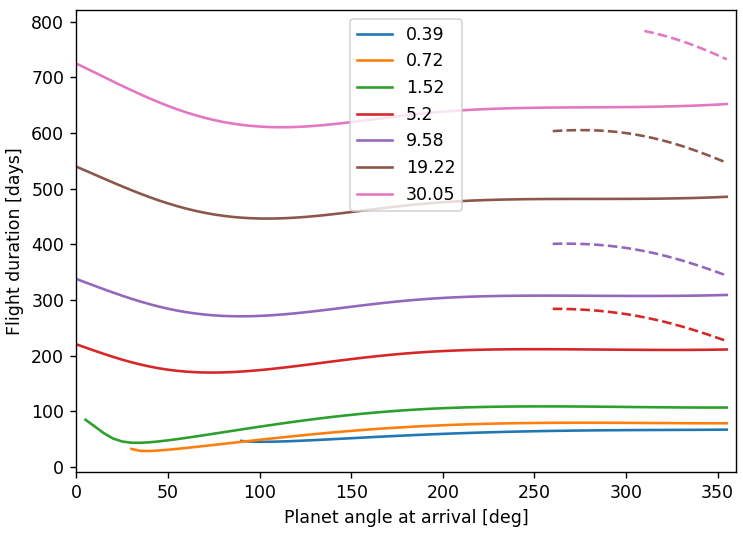
\includegraphics[width=\linewidth]{article_003.png}
    \caption{Flight times in days versus final polar angle at arrival.}
    \label{fig:final_theta}
\end{figure}
\begin{figure}[htbp]
    \centering
    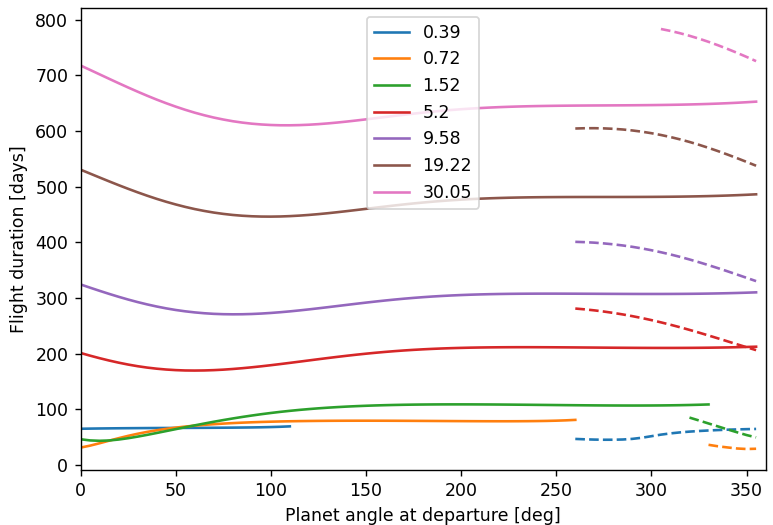
\includegraphics[width=\linewidth]{article_004.png}
    \caption{Flight times in days versus initial polar angle at departure.}
    \label{fig:starting_theta}
\end{figure}

\begin{figure*}[p]
    \centering
    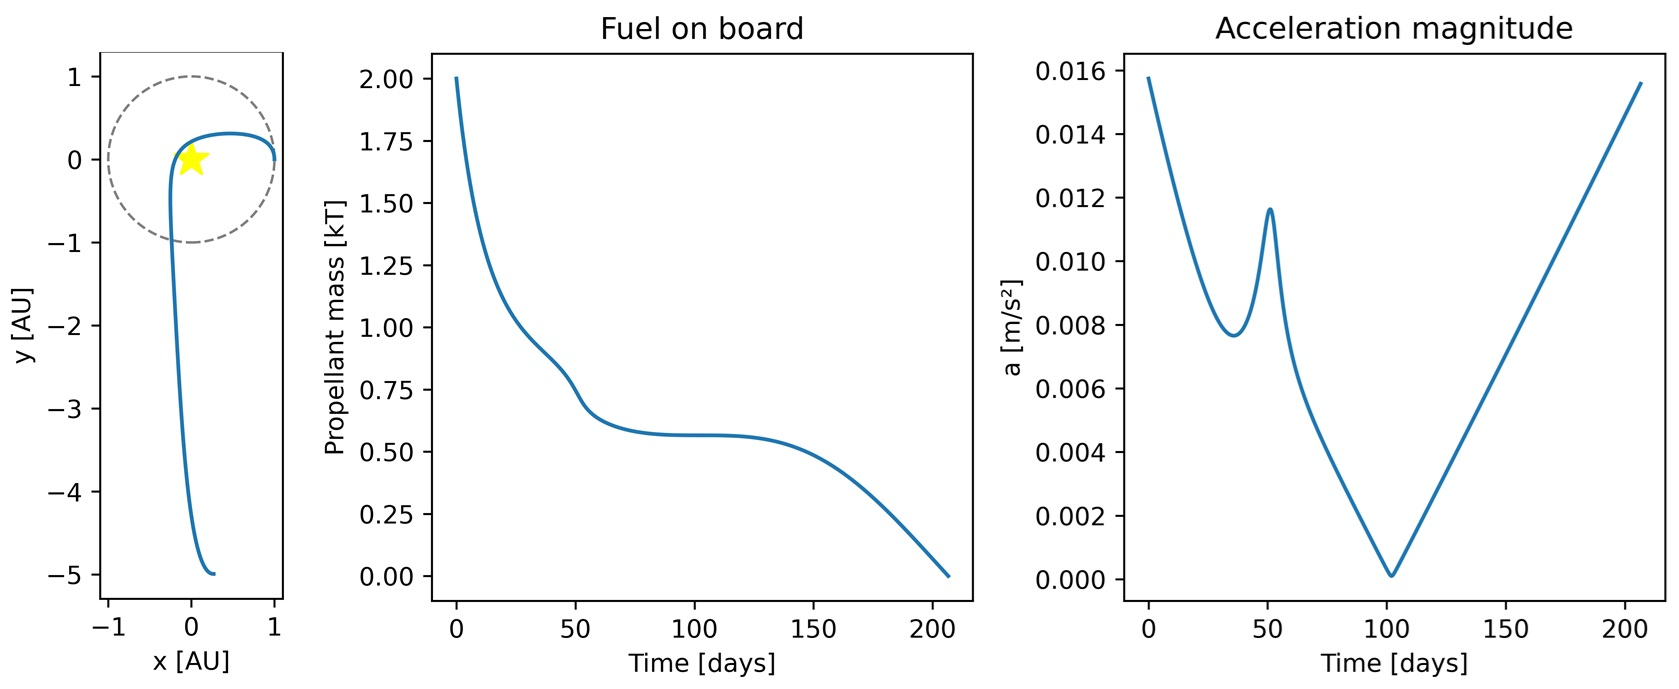
\includegraphics[width=0.75\linewidth]{article_001.jpg}
    \caption{Example trajectory from $r=1$\,AU, $\theta=0^\circ$ to $r=5$\,AU, $\theta=273.1^\circ$ in 207 days. The trajectory includes a low-perihelion Oberth-like pass to gain orbital energy, which is apparent from the acceleration peak around day 50.}
    \label{fig:oberth_figure}
\end{figure*}
\begin{figure*}[p]
    \centering
    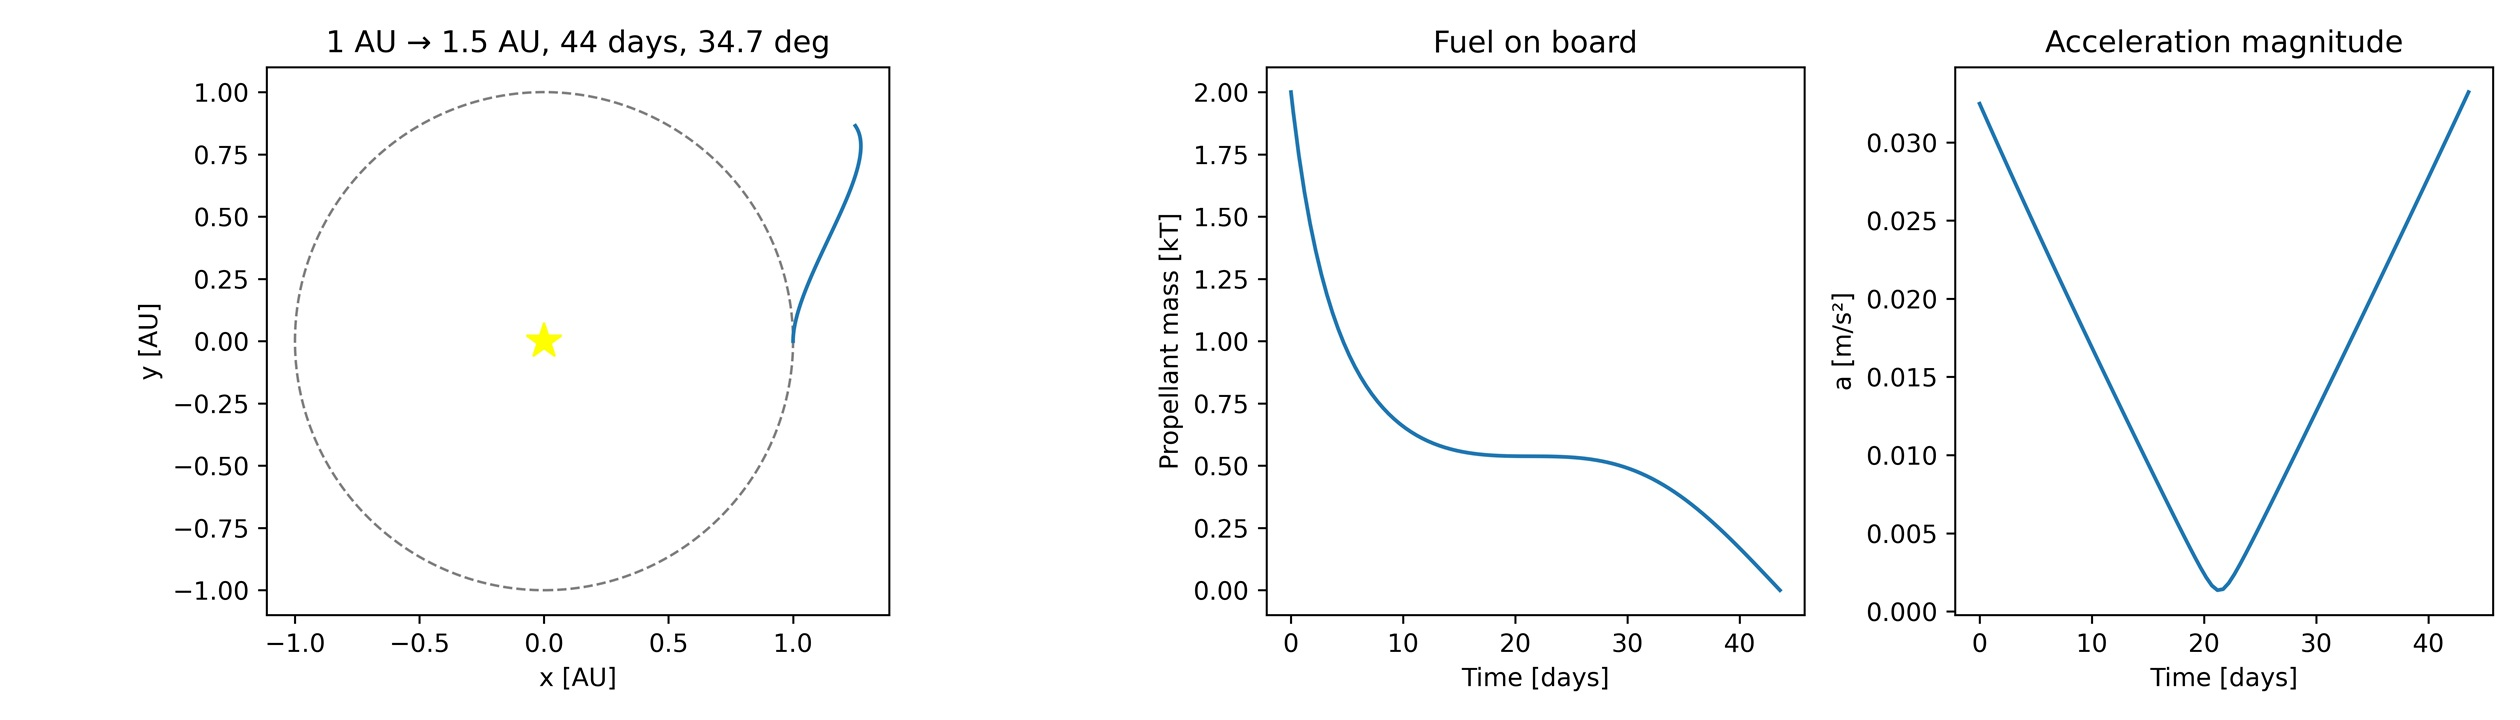
\includegraphics[width=\linewidth]{article_005.jpg}
    \caption{Example trajectory from $r=1$\,AU, $\theta=0^\circ$ to $r=1.5$\,AU, $\theta=34.7^\circ$ in 44 days. Recomputing the stated rounded geometry gives 42.55 days (Sec.~\ref{sec:diagnostics}), so the plotted path is not reproduced exactly.}
    \label{fig:non_oberth_figure}
\end{figure*}
\begin{figure*}[p]
    \centering
    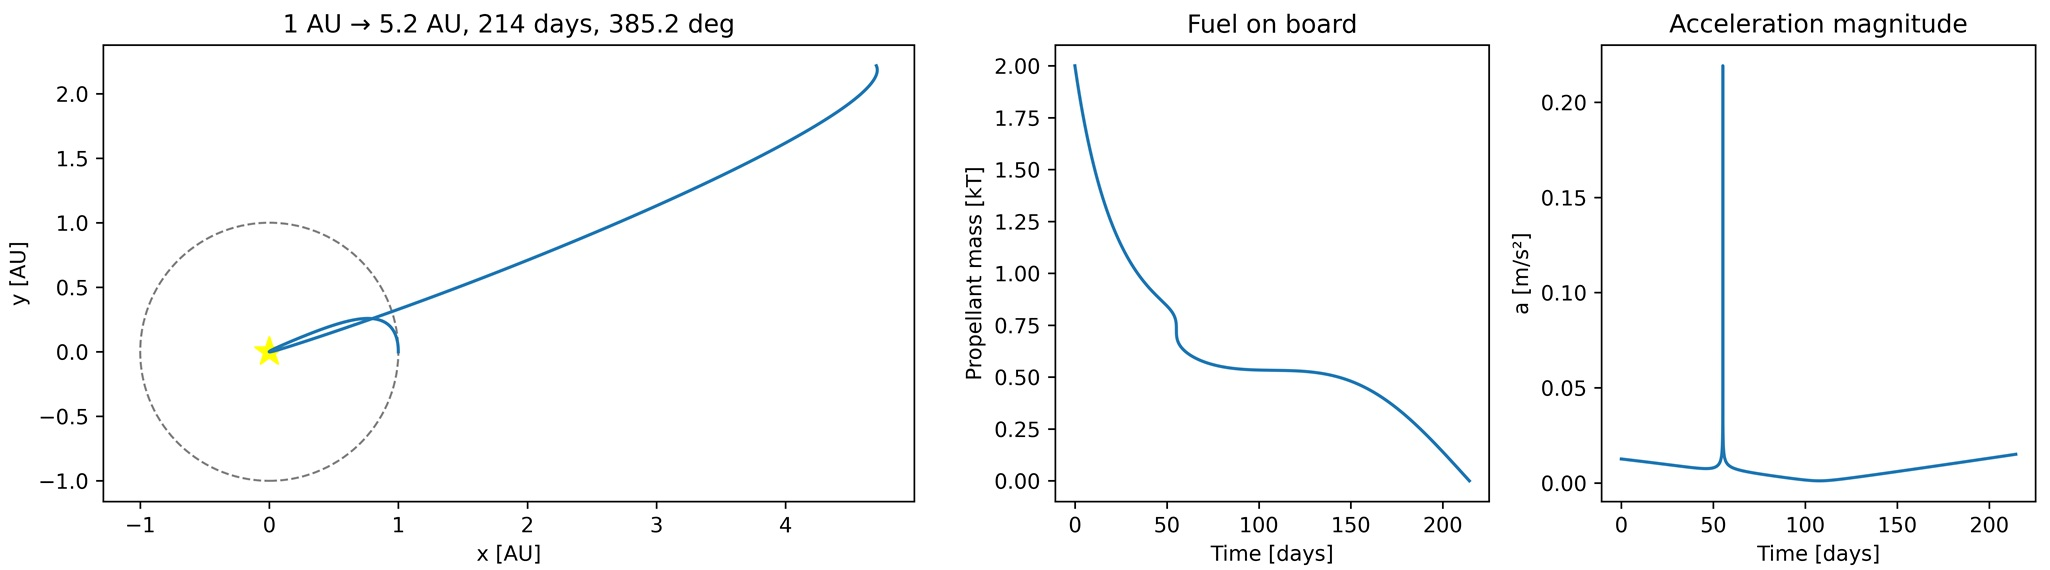
\includegraphics[width=\textwidth]{article_002.jpg}
    \caption{An example of a more extreme low-perihelion Oberth-like maneuver for a transfer to Jupiter's orbit. The trajectory is from $r=1$\,AU, $\theta=0^\circ$ to $r=5.2$\,AU, $\theta=385.2^\circ$ and lasts 214 days. Its $0.00027$\,AU perihelion lies inside the Sun, so it illustrates the unconstrained model rather than a feasible mission; the $\Theta=25^\circ$ winding class reaches nearly the same terminal state in 193 days without a solar pass.}
    \label{fig:oberth_figure2}
\end{figure*}


\FloatBarrier

\section*{Acknowledgment}
The author wishes to acknowledge the use of large language models (Google's Gemini and OpenAI's GPT) for assistance in improving the language and clarity of the manuscript, for aiding in the implementation of the numerical code and derivations of some of the analytical results. The results were tested and verified by the author.


\appendices
\section{Finite-Ceiling Free-Space Derivation}
\label{sec:appendix_capped_derivation}
For the dimensional time problem in one dimension, let
$l=\lambda_v$ with $l'=-\lambda_x$ and $\lambda_x$ constant.
On a powered fixed-sign interval, write $|l|=L_a+nt$.
For fixed exhaust $V$ set $F=2P/V$, $\sigma=2P/V^2$ and
$C_m=\lambda_m m^2$. Differentiating the optimized Hamiltonian gives
\begin{equation}
 m'=-\sigma,\quad
 \lambda_m'=\frac{F|l|}{m^2},\quad
 C_m'=\frac{2P|l|}{V}-\frac{4PC_m}{mV^2}.
\end{equation}
Thus $C_m$ is not constant on this boundary. With
$B=n/\sigma$ and $A=L_a+Bm_a$,
\begin{equation}
 \begin{gathered}
 m=m_a-\sigma t,\\
 \lambda_m=\lambda_{m,a}
 +V\left[A\left(\frac1m-\frac1{m_a}\right)
                  +B\log\frac m{m_a}\right].
 \end{gathered}
\end{equation}
For thrust sign $\epsilon=\pm1$,
\begin{equation}
 \begin{split}
 v&=v_a+\epsilon V\log(m_a/m),\\
 x&=x_a+v_at+\epsilon V
                \left[t-\frac m\sigma\log(m_a/m)\right].
 \end{split}
\end{equation}
On an ideal interior arc $C_m$ is constant and $a=Pl/C_m$;
on a coast both $m$ and $\lambda_m$ are constant.

\subsection{Relations carried over from the uncapped analysis}
The pointwise selector holds when evaluated with the current $C_m$.
The fixed-exhaust state maps above, the interior-arc mass formula, and
the exchange argument excluding an avoidable powered--coast rearrangement
under its monotone braking hypotheses also hold. On an interior arc
$l=l_a-nt$,
\begin{equation}
 \frac1{m(t)}=\frac1{m_a}+\frac{P}{2C_m^2}
       (l_a^2t-l_an t^2+n^2t^3/3).
\end{equation}
Integrating $a=Pl/C_m$ gives quadratic velocity and cubic position.
The raw primer remains affine globally; its scaled acceleration does not.
Because $C_m$ varies on boundary arcs, switching times cannot be
obtained from a constant-$C_m$ primer, not even with its terminal value.

\begin{lemma}[Coast/boundary exchange]
In a monotone nonnegative-velocity braking phase, any positive coast after a positive fixed-exhaust brake can be moved ahead of the burns and shortened to preserve distance, terminal velocity and mass while reducing time.
\end{lemma}
\begin{proof} In a
coast/ceiling-brake mixture with duty fraction $\delta\in[0,1]$, write
$s(t)=\int\delta\,dt$. Then $m=m_a-\sigma s$ and
$v=v_a-V\log(m_a/m)$. Final mass and velocity depend only on total
powered time. Exchanging a burn followed by a coast of length $c$ for
coast followed by burn increases distance by $c\,\Delta v>0$, where
$\Delta v$ is the burn's velocity decrement. Repetition puts all coasting
first. If the braking interval has $0\le v\le v_a$ and $v_a>0$, its
original coast distance is reproduced by a shorter leading coast of
duration $\int_{\rm coast}v\,dt/v_a$. Mass, terminal velocity and distance
are unchanged, while elapsed time strictly decreases whenever a positive
coast follows a positive brake. Approximation extends this state argument
to fractional mixtures. The argument uses only the state equations.
\end{proof}

\subsection{Ceiling-only topology and the unresolved two-sided case}
Consider the ceiling-only, positive-distance, rest-to-rest problem with
$C_m>0$ and positive dry mass. Normalize the constant $\lambda_x=n>0$;
the primer is $l=n(t_z-t)$. Define
$z=Vm|l|/(2C_m)$. The selector gives interior $\mathsf U$ for $z>1$,
ceiling burn $\mathsf B$ for $1/2<z<1$, and coast $\mathsf C$ for $z<1/2$.
On a ceiling arc,
\begin{equation}
 \frac{z'}z=\frac{|l|'}{|l|}+\frac{\sigma}{m}(1-2z),
 \qquad \sigma=2P/V^2.
\end{equation}
On an interior arc $z'/z=|l|'/|l|-\sigma z^2/m$; on a coast it is
$|l|'/|l|$. During boost $|l|'<0$, so $z$ decreases strictly through
$\mathsf U_+,\mathsf B_+,\mathsf C$, with initial truncations allowed.
On braking $|l|'=n>0$. At $z=1/2$ both the coast and boundary vector
fields have $z'>0$. Thus $\mathsf C\to\mathsf B_-$ is regular and cannot
return to the tie: every encounter with that level would point upward.
No sliding arc or terminal $m_6$ event is available.

At $z=1$ both powered fields give
$z'/z=n/|l|-\sigma/m$. The quantity
$k=mn/(\sigma|l|)$ decreases strictly throughout braking, since $m$
decreases and $|l|$ increases. An upward crossing $\mathsf B_-\to\mathsf U_-$
can occur only while $k>1$, and a subsequent downward crossing
$\mathsf U_-\to\mathsf B_-$ only when $k<1$; no further reversal is
possible. Consequently every such finite-switch normal candidate has
the ordered pattern
\begin{equation}
 \mathsf U_+\;\mathsf B_+\;\mathsf C\;\mathsf B_-\;
 \mathsf U_-\;\mathsf B_-,
\end{equation}
with absent intervals and endpoint truncations permitted. In particular
the last boundary burn ends at the endpoint, not at a return to coast.
This is a ceiling-only one-dimensional result. For the two-sided
$50$--$250$ km/s engine, the $50$ km/s lower exhaust limit caps
acceleration and introduces additional arcs.

To state precisely what remains unresolved here, write $V_-=50$ km/s,
$V_+=250$ km/s, $\rho_V=V_+/V_-=5$, and define $z$ with $V=V_+$.
For $C_m>0$, the dimensional selector becomes
\begin{equation}
 |a|=\begin{cases}
 0,&z<1/2,\\
 2P/(mV_+),&1/2<z<1,\\
 P|l|/C_m,&1<z<\rho_V,\\
 2P/(mV_-),&z>\rho_V.
 \end{cases}
\end{equation}
The last region is a maximum-acceleration ($a_+$) arc, denoted
$\mathsf A_\pm$ according to thrust sign. Its state and mass-adjoint
maps are the fixed-exhaust maps above with $V=V_-$, and
\begin{equation}
 \frac{z'}z=\frac{|l|'}{|l|}
   +\frac{\sigma_-}{m}\left(1-\frac{2z}{\rho_V}\right),
 \qquad\sigma_-=2P/V_-^2.
\end{equation}
Thus the selector and propagation are available for both boundaries,
but a complete two-sided switching-topology theorem, including all
$\mathsf A_\pm$ visits and admissible endpoint truncations, is left open,
as are gravity, abnormal extremals and other endpoint conditions.

\subsection{Endpoint reduction}
This reduction and its numerical fixture retain the ceiling-only
assumptions of the proved topology.
Use homogeneity to fix $n=1$. The two shooting unknowns are $t_z$ and
$\lambda_m(0)>0$. Propagate the exact interior, boundary and coast maps,
switching with the current $z$, until the first exhaustion $m=m_d$.
Call that time $T(t_z,\lambda_m(0))$. Solve
\begin{equation}
 x(T;t_z,\lambda_m(0))=L,\qquad
 v(T;t_z,\lambda_m(0))=0.
\end{equation}
Reject trajectories without exhaustion or with invalid adjoint sign or
switch inequalities. Alternatively use $T$ as a third unknown and add
$m(T)=m_d$ as a third residual. Normalize the free-time Hamiltonian
afterward if a positive normal scaling exists, and compare competing
solutions, since the reduction does not imply uniqueness.

For $P=1/2$, $V=2$, $m_0=1$, $m_d=1/2$, $L=1$, independent numerical
integration of the selector gives
$t_z=1.22365494$, $\lambda_m(0)=0.61524660$, $T=2.35199587$;
the maximum endpoint residual is $9.6\,10^{-8}$. The coast is approximately
$[0.80144,1.64581]$. Direct transcription with piecewise-constant
acceleration, exact $(x,v,1/m)$ propagation and the ceiling imposed at
each burn cell's final mass gives:
\begin{center}\begin{tabular}{rrr}\toprule
Burn cells&Time&Endpoint error\\\midrule
12&2.35489579&$2.6\,10^{-12}$\\
24&2.35338380&$1.4\,10^{-12}$\\
48&2.35267314&$1.3\,10^{-12}$\\\bottomrule
\end{tabular}\end{center}
The within-cell ceiling holds because inverse mass increases monotonically
and the acceleration is constant. Ceiling violations at optimizer tolerance
are below $9\,10^{-13}$. The transcription independently checks the
trajectory equations and approaches the shooting time from above.


\section{Power-System Mass Closure for the Free-Space Benchmark}
\label{sec:appendix_mass_closure}

The benchmark result \eqref{eq:Tmin} was derived for prescribed initial and dry masses.
For high-power spacecraft, however, the dry mass may itself depend on the propulsion system, because both the power-conversion hardware and the radiators must be carried together with the payload.
This appendix shows how the free-space minimum-time law is modified under a simple power-system mass closure.

Let \(P\) denote the useful jet power appearing in the rocket model, and let \(P_\mathrm{tot}\) be the total onboard engine power.
Define
\begin{equation}
  \alpha_\mathrm{eng} \equiv \frac{P_\mathrm{tot}}{m_\mathrm{eng}},
  \qquad
  \phi \equiv \frac{P_\mathrm{heat}}{P_\mathrm{tot}},
  \qquad
  \rho_\mathrm{rad} \equiv \frac{P_\mathrm{heat}}{m_\mathrm{rad}},
\end{equation}
where \(\alpha_\mathrm{eng}\) is the engine specific power, \(\phi\) is the waste-heat fraction, and \(\rho_\mathrm{rad}\) is the radiator specific heat-rejection capability.
Since only the fraction \(1-\phi\) of the total power is converted into useful jet power,
\begin{equation}
  P = (1-\phi)P_\mathrm{tot},
  \qquad
  P_\mathrm{heat} = \phi P_\mathrm{tot}
  = \frac{\phi}{1-\phi}P.
\end{equation}
Therefore,
\begin{equation}
  m_\mathrm{eng}=\frac{P}{(1-\phi)\alpha_\mathrm{eng}},
  \qquad
  m_\mathrm{rad}=\frac{\phi}{1-\phi}\frac{P}{\rho_\mathrm{rad}}.
\end{equation}

Let \(m_\mathrm{pay}\) be the payload mass.
The dry mass can then be written in the affine form
\begin{equation}
  m_\mathrm{dry}=m_\mathrm{pay}+m_\mathrm{eng}+m_\mathrm{rad}
  = m_\mathrm{pay}+\beta P,
  \label{eq:mdry_beta_app}
\end{equation}
with
\begin{equation}
  \beta \equiv
  \frac{1}{(1-\phi)\alpha_\mathrm{eng}}
  +\frac{\phi}{(1-\phi)\rho_\mathrm{rad}}.
  \label{eq:beta_def_app}
\end{equation}
The quantity \(\beta\) has units of kg/W and is the inverse of the effective propulsion-system specific power,
\begin{equation}
  \alpha_\mathrm{sys}\equiv \beta^{-1}.
\end{equation}

To close the mass model, assume a fixed fuel-to-dry-mass ratio
\begin{equation}
  \mathcal{R}\equiv \frac{m_\mathrm{fuel}}{m_\mathrm{dry}}.
\end{equation}
Then
\begin{equation}
  m_i=(1+\mathcal{R})m_\mathrm{dry},
\end{equation}
and the parameter \(\Delta\) from \eqref{eq:Tmin} becomes
\begin{equation}
  \Delta
  = \frac{1}{m_\mathrm{dry}}-\frac{1}{m_i}
  = \frac{\mathcal{R}}{(1+\mathcal{R})m_\mathrm{dry}}.
  \label{eq:Delta_payload_app}
\end{equation}
Substituting \eqref{eq:mdry_beta_app} and \eqref{eq:Delta_payload_app} into the benchmark law \eqref{eq:Tmin} yields
\begin{equation}
  T(P)
  =
  \left[
    \frac{6L^2(1+\mathcal{R})}{\mathcal{R}}
    \left(
      \frac{m_\mathrm{pay}}{P}+\beta
    \right)
  \right]^{1/3}.
  \label{eq:T_payload_beta_app}
\end{equation}
Equation~\eqref{eq:T_payload_beta_app} is the free-space minimum-time law when the dry mass is allowed to scale linearly with propulsion power.

Several immediate consequences follow.
First,
\begin{equation}
  T^3(P)
  =
  \frac{6L^2(1+\mathcal{R})}{\mathcal{R}}
  \left(
    \frac{m_\mathrm{pay}}{P}+\beta
  \right),
\end{equation}
so that
\begin{equation}
  \frac{d}{dP}T^3(P)
  =
  -\frac{6L^2(1+\mathcal{R})}{\mathcal{R}}
   \frac{m_\mathrm{pay}}{P^2}
  <0.
\end{equation}
Under the idealized assumptions of this closure---unlimited exhaust speed, fixed waste-heat fraction \(\phi\), fixed engine specific power \(\alpha_\mathrm{eng}\), and fixed radiator specific heat rejection \(\rho_\mathrm{rad}\), all independent of operating point---the transfer time decreases monotonically with power and has no finite mathematical optimum:
\begin{equation}
  P^\star \to \infty.
\end{equation}
This formal limit should not be interpreted as a physically achievable design target, since at very large \(P\) the assumed linear mass closure breaks down: in practice \(\rho_\mathrm{rad}\) depends on the radiator operating temperature, \(\alpha_\mathrm{eng}\) is bounded by materials and shielding, and the exhaust speed itself is bounded above. The relevant practical implication is rather the second observation: the family approaches the asymptotic lower bound
\begin{equation}
  T_\infty
  =
  \left[
    \frac{6L^2(1+\mathcal{R})}{\mathcal{R}}\,\beta
  \right]^{1/3}.
  \label{eq:T_infty_beta_app}
\end{equation}
This lower bound arises because increasing \(P\) also increases the dry mass that must be accelerated.

A convenient engineering scale is obtained by equating propulsion-hardware mass to payload mass,
\begin{equation}
  m_\mathrm{eng}+m_\mathrm{rad}=m_\mathrm{pay}.
\end{equation}
Using \eqref{eq:mdry_beta_app}, this defines the characteristic power
\begin{equation}
  \beta P_\mathrm{knee}=m_\mathrm{pay},
  \qquad
  P_\mathrm{knee}=\frac{m_\mathrm{pay}}{\beta}
  = \alpha_\mathrm{sys}m_\mathrm{pay}.
  \label{eq:Pknee_app}
\end{equation}
At this point the dry mass is \(m_\mathrm{dry}=2m_\mathrm{pay}\), and \eqref{eq:T_payload_beta_app} can be written as
\begin{equation}
  T(P)=T_\infty
  \left(
    1+\frac{P_\mathrm{knee}}{P}
  \right)^{1/3}.
  \label{eq:T_knee_form_app}
\end{equation}
Hence
\begin{equation}
  T(P_\mathrm{knee}) = 2^{1/3}T_\infty.
  \label{eq:Tknee_app}
\end{equation}

Equations~\eqref{eq:T_payload_beta_app}--\eqref{eq:Tknee_app} provide an engineering interpretation of the free-space benchmark.
They are not used in the subsequent Sun-field optimal-control formulation, but they show how the cubic-root time law is modified when propulsion-system mass scales with power.

\section{Direct Method Using Spline Parameterization}

\label{sec:appendix}
Before adopting the indirect method based on Pontryagin's Maximum Principle (PMP) detailed in the main body of this paper, a more straightforward \emph{direct method} was explored. Direct methods seek to find the optimal trajectory by parameterizing the path with a set of functions and then using a nonlinear programming solver to find the best parameters. This approach avoids the complexity of deriving and solving the costate equations.

Our implementation parameterized the spacecraft's trajectory, $\mathbf{r}(t) = (x(t), y(t))$, using cubic splines. The core idea is to define the path by a small number of control points, which become the variables for optimization.

The procedure was as follows:
{
\renewcommand{\labelenumi}{\arabic{enumi}.}
\begin{enumerate}
    \item A fixed number of $N$ control points, $(\mathbf{p}_i, t_i)$ for $i=0, \dots, N-1$, were defined along the time axis of the transfer. The endpoints, $\mathbf{p}_0$ and $\mathbf{p}_{N-1}$, were fixed to match the start and end positions of the transfer arc. The initial and final velocities were enforced by connecting the transfer arc to the initial and final circular orbits.
    \item The positions of the intermediate $N-2$ control points were the free variables for the optimization.
    \item For any given set of control points, two cubic splines, $x_s(t)$ and $y_s(t)$, were fitted to create a continuous and smooth trajectory $\mathbf{r}(t) = (x_s(t), y_s(t))$. A cubic spline is defined piecewise by third-order polynomials, ensuring that the first and second derivatives (velocity and acceleration) are continuous across the entire path.
    \item The required velocity $\dot{\mathbf{r}}(t)$ and acceleration $\ddot{\mathbf{r}}(t)$ vectors were obtained by numerically differentiating the spline functions.
    \item With the total acceleration $\ddot{\mathbf{r}}(t)$ known, the required thrust acceleration was calculated by subtracting the gravitational component:
    \begin{equation}
        \mathbf{a}_T(t) = \ddot{\mathbf{r}}(t) - \mathbf{a}_g(\mathbf{r}(t)).
    \end{equation}
    \item The instantaneous mass flow rate was then determined from the thrust acceleration magnitude using \eqref{eq:mass_flow}. Integrating this rate backwards in time yielded the total propellant consumed for the maneuver.
    \item A nonlinear optimizer (specifically, the Nelder--Mead method) was used to adjust the positions of the intermediate control points to minimize a cost function based on the final fuel expenditure and flight time.
\end{enumerate}
}

\subsection*{Limitations and Stagnation in Local Minima}
While conceptually simple, this direct method proved inadequate for finding high-performance trajectories. The primary difficulty was the nature of the optimization landscape. The relationship between the position of a control point and the final mission cost is highly complex and nonlinear. As a result, the search space is filled with a vast number of local minima.

For a very small number of intermediate control points ($N=3$ or $N=4$ total), the method could find a reasonable, smooth trajectory. However, as the number of control points was increased to grant the path more freedom and potential for higher performance, the dimensionality of the search space grew, and the solver would invariably become trapped in a suboptimal local minimum.

An attempt was made to mitigate this by using a continuation strategy on the number of control points: first, an optimal path with $N=4$ points was found. Then, a fifth point was added at the location of maximum curvature, and the system was re-optimized. While this yielded marginal improvements, the solution quality consistently stagnated far below that achievable with the PMP-based method. The direct spline method lacks the rigorous guidance provided by the costate (or "primer vector") variables, which point the way toward optimality across the entire trajectory. These difficulties ultimately motivated the adoption of the indirect shooting method presented in this work.

\bibliographystyle{ieeetr}

\bibliography{KeplerVariableISPReferences}

%\begin{table*}[!htbp]
\footnotesize\renewcommand{\arraystretch}{0.9}
%\centering
%\caption{Transfer time in days found by the solver (U: unresolved) to a circular orbit of a given %radius and final polar angle.}
%\label{tab:transfer_times}
%\sisetup{table-format=3.2}
%\begin{tabular}{r S S S S S S S S}
%\toprule
%\textbf{Polar Angle} & \multicolumn{8}{c}{\textbf{Target Radius (AU)}} %\\
%\cmidrule(lr){2-9}
%\textbf{(\si{\degree})} & {0.3} & {0.75} & {1.643} & {3} & {5} & {10} & %{15} & {20} \\
%\midrule
%-100 & {U} & {U} & 172.79 & 214.70 & 278.24 & 411.05 & 521.03 & 617.79 \\
%-95  & {U} & {U} & 172.53 & 214.38 & 278.09 & 411.36 & 521.71 & 618.81 \\
%-90  & {U} & {U} & 172.04 & 213.82 & 277.69 & 411.37 & 522.08 & 619.49 \\
%-85  & {U} & {U} & 171.31 & 213.01 & 277.01 & 411.07 & 522.09 & 619.81 \\
%-80  & {U} & {U} & 170.30 & 211.89 & 276.00 & 410.38 & 521.69 & 619.66 \\
%-75  & {U} & {U} & 169.02 & 210.48 & 274.68 & 409.32 & 520.91 & 619.10 \\
%-70  & {U} & {U} & 167.45 & 208.77 & 273.04 & 407.90 & 519.68 & 618.09 \\
%-65  & {U} & {U} & 165.56 & 206.75 & 271.06 & 406.11 & 518.00 & 616.62 \\
%-60  & {U} & {U} & 163.31 & 204.37 & 268.70 & 403.85 & 515.90 & 614.62 \\
%-55  & {U} & {U} & 160.72 & 201.64 & 265.98 & 401.20 & 513.34 & 612.07 \\
%-50  & {U} & {U} & 157.75 & 198.53 & 262.91 & 398.15 & 510.26 & 609.06 \\
%-45  & {U} & {U} & 154.36 & 195.05 & 259.48 & 394.69 & 506.73 & 605.55 \\
%-40  & {U} & {U} & 150.51 & 191.19 & 255.65 & 390.78 & 502.75 & 601.49 \\
%-35  & {U} & {U} & 146.19 & 186.97 & 251.46 & 386.49 & 498.35 & 596.95 \\
%-30  & {U} & {U} & 141.39 & 182.31 & 246.95 & 381.83 & 493.47 & 591.90 \\
%-25  & {U} & {U} & 136.01 & 177.29 & 242.13 & 376.83 & 488.23 & 586.47 \\
%-20  & {U} & {U} & 129.99 & 171.93 & 236.97 & 371.49 & 482.60 & 580.58 \\
%-15  & {U} & {U} & 123.33 & 166.21 & 231.57 & 365.86 & 476.66 & 574.36 \\
%-10  & {U} & {U} & 115.97 & 160.22 & 225.98 & 360.03 & 470.45 & 567.80 \\
%-5   & {U} & {U} & 107.80 & 154.01 & 220.23 & 354.01 & 464.02 & 560.98 \\
%0    & {U} & {U} & 98.73  & 147.65 & 214.39 & 347.87 & 457.41 & 553.97 \\
%5    & {U} & {U} & 88.85  & 141.28 & 208.56 & 341.66 & 450.70 & 546.83 \\
%10   & {U} & {U} & 78.39  & 135.03 & 202.80 & 335.46 & 443.96 & 539.61 \\
%15   & {U} & {U} & 68.14  & 129.05 & 197.20 & 329.34 & 437.24 & 532.38 \\
%20   & {U} & {U} & 59.71  & 123.57 & 191.88 & 323.36 & 430.63 & 525.22 \\
%25   & {U} & {U} & 54.06  & 118.69 & 186.91 & 317.60 & 424.16 & 518.19 \\
%30   & {U} & 27.24 & 51.06  & 114.50 & 182.34 & 312.10 & 417.94 & 511.36 \\
%35   & {U} & 26.78 & 50.12  & 111.06 & 178.22 & 306.91 & 412.01 & 504.81 \\
%40   & {U} & 27.70 & 50.34  & 108.50 & 174.68 & 302.14 & 406.39 & 498.55 \\
%45   & {U} & 29.08 & 51.39  & 106.67 & 171.68 & 297.78 & 401.14 & 492.63 \\
%50   & {U} & 30.74 & 52.90  & 105.51 & 169.21 & 293.85 & 396.35 & 487.18 \\
%55   & {U} & 32.52 & 54.76  & 104.96 & 167.26 & 290.38 & 392.01 & 482.16 \\
%60   & {U} & 34.39 & 56.87  & 104.98 & 165.89 & 287.44 & 388.13 & 477.60 \\
%65   & {U} & 36.30 & 59.12  & 105.46 & 165.00 & 284.97 & 384.75 & 473.51 \\
%70   & {U} & 38.25 & 61.48  & 106.30 & 164.55 & 282.97 & 381.85 & 469.98 \\
%75   & {U} & 40.20 & 63.90  & 107.45 & 164.50 & 281.41 & 379.42 & 466.92 \\
%80   & {U} & 42.15 & 66.38  & 108.91 & 164.86 & 280.36 & 377.53 & 464.42 \\
%85   & {U} & 44.09 & 68.87  & 110.55 & 165.54 & 279.72 & 376.11 & 462.41 \\
%90   & {U} & 46.02 & 71.37  & 112.40 & 166.54 & 279.47 & 375.11 & 460.87 \\
%95   & {U} & 47.92 & 73.86  & 114.37 & 167.78 & 279.58 & 374.54 & 459.79 \\
%100  & {U} & 49.80 & 76.32  & 116.45 & 169.24 & 280.07 & 374.41 & 459.18 \\
%105  & {U} & 51.65 & 78.76  & 118.62 & 170.87 & 280.86 & 374.65 & 458.98 \\
%110  & {U} & 53.46 & 81.15  & 120.84 & 172.69 & 281.91 & 375.21 & 459.21 \\
%115  & {U} & 55.23 & 83.49  & 123.09 & 174.61 & 283.20 & 376.08 & 459.77 \\
%120  & {U} & 56.96 & 85.77  & 125.35 & 176.62 & 284.72 & 377.25 & 460.65 \\
%125  & {U} & 58.64 & 88.00  & 127.60 & 178.70 & 286.41 & 378.65 & 461.81 \\
%130  & 48.33 & 60.28 & 90.14  & 129.82 & 180.82 & 288.22 & 380.23 & 463.22 \\
%135  & 48.34 & 61.86 & 92.20  & 132.00 & 182.95 & 290.14 & 381.98 & 464.84 \\
%140  & 48.55 & 63.38 & 94.18  & 134.12 & 185.06 & 292.14 & 383.87 & 466.63 \\
%145  & 48.89 & 64.83 & 96.07  & 136.17 & 187.15 & 294.18 & 385.84 & 468.54 \\
%150  & 49.33 & 66.23 & 97.85  & 138.13 & 189.18 & 296.23 & 387.87 & 470.53 \\
%155  & 49.84 & 67.57 & 99.54  & 139.99 & 191.14 & 298.25 & 389.91 & 472.58 \\
%160  & 50.39 & 68.83 & 101.12 & 141.74 & 193.00 & 300.22 & 391.94 & 474.63 \\
%165  & 50.97 & 70.03 & 102.60 & 143.39 & 194.76 & 302.13 & 393.92 & 476.66 \\
%170  & 51.58 & 71.15 & 103.97 & 144.91 & 196.41 & 303.94 & 395.83 & 478.65 \\
%175  & 52.20 & 72.21 & 105.23 & 146.30 & 197.92 & 305.65 & 397.64 & 480.54 \\
%180  & 52.81 & 73.20 & 106.38 & 147.58 & 199.32 & 307.22 & 399.34 & 482.33 \\
%185  & 53.43 & 74.12 & 107.42 & 148.73 & 200.58 & 308.66 & 400.93 & 484.00 \\
%190  & 54.04 & 74.97 & 108.37 & 149.75 & 201.70 & 309.97 & 402.35 & 485.55 \\
%195  & 54.64 & 75.75 & 109.21 & 150.66 & 202.69 & 311.14 & 403.64 & 486.93 \\
%200  & 55.23 & 76.47 & 109.95 & 151.45 & 203.55 & 312.15 & 404.78 & 488.18 \\
%205  & 55.80 & 77.13 & 110.60 & 152.13 & 204.30 & 313.04 & 405.79 & 489.27 \\
%210  & 56.35 & 77.72 & 111.16 & 152.70 & 204.93 & 313.80 & 406.65 & 490.23 \\
%215  & 56.88 & 78.25 & 111.65 & 153.19 & 205.45 & 314.44 & 407.39 & 491.06 \\
%220  & 57.39 & 78.72 & 112.04 & 153.58 & 205.87 & 314.97 & 408.01 & 491.77 \\
%225  & 57.87 & 79.14 & 112.38 & 153.91 & 206.21 & 315.39 & 408.53 & 492.35 \\
%230  & 58.34 & 79.51 & 112.64 & 154.14 & 206.47 & 315.73 & 408.94 & 492.83 \\
%235  & 58.78 & 79.83 & 112.85 & 154.31 & 206.66 & 316.00 & 409.27 & 493.22 \\
%240  & 59.20 & 80.10 & 113.00 & 154.43 & 206.79 & 316.18 & 409.52 & 493.54 \\
%245  & 59.60 & 80.33 & 113.10 & 154.49 & 206.86 & 316.30 & 409.70 & 493.78 \\
%250  & 59.97 & 80.50 & 113.15 & 154.51 & 206.88 & 316.38 & 409.84 & 493.96 \\
%255  & 60.32 & 80.65 & 113.16 & 154.49 & 206.86 & 316.41 & 409.92 & 494.09 \\
%260  & 60.65 & 80.76 & 113.13 & 154.43 & 206.80 & 316.41 & 409.96 & 494.18 \\
%265  & 60.97 & 80.83 & 113.07 & 154.34 & 206.73 & 316.37 & 409.97 & 494.24 \\
%270  & 61.25 & 80.86 & 112.99 & 154.23 & 206.63 & 316.31 & 409.96 & 494.27 \\
%\bottomrule
%\end{tabular}
%\end{table*}



\begin{table*}[tbp]
\footnotesize\renewcommand{\arraystretch}{0.9}
\centering
\footnotesize
\renewcommand{\arraystretch}{0.9}
\caption{Transfer time in days found by the solver (U: unresolved) from a circular orbit of 1 AU and final polar angle (at rocket arrival).}
\label{tab:transfer_times_final_anomaly}
\sisetup{table-format=3.2} % Requires siunitx LaTeX package
\begin{tabular}{{r S S S S S S S }}
\toprule
\textbf{Polar angle} & \multicolumn{7}{c}{\textbf{Target Radius (AU)}} \\
\cmidrule(lr){2-8}
\textbf{(\si{\degree})} & {0.390} & {0.720} & {1.520} & {5.200} & {9.580} & {19.220} & {30.050} \\
\midrule
0 & {U} & {U} & {U} & 220.50 & 337.82 & 539.55 & 724.65 \\
5 & {U} & {U} & 84.99 & 214.66 & 331.66 & 532.47 & 716.76 \\
10 & {U} & {U} & 73.01 & 208.91 & 325.52 & 525.31 & 708.75 \\
15 & {U} & {U} & 60.88 & 203.32 & 319.44 & 518.17 & 700.69 \\
20 & {U} & {U} & 51.35 & 197.98 & 313.53 & 511.09 & 692.64 \\
25 & {U} & {U} & 45.94 & 192.95 & 307.83 & 504.13 & 684.71 \\
30 & {U} & 32.66 & 43.80 & 188.35 & 302.40 & 497.40 & 676.93 \\
35 & {U} & 29.03 & 43.63 & 184.23 & 297.29 & 490.93 & 669.37 \\
40 & {U} & 28.92 & 44.61 & 180.59 & 292.59 & 484.76 & 662.08 \\
45 & {U} & 29.86 & 46.15 & 177.47 & 288.32 & 478.95 & 655.19 \\
50 & {U} & 31.19 & 48.07 & 174.94 & 284.48 & 473.58 & 648.68 \\
55 & {U} & 32.74 & 50.23 & 172.94 & 281.10 & 468.66 & 642.60 \\
60 & {U} & 34.42 & 52.55 & 171.44 & 278.25 & 464.20 & 637.00 \\
65 & {U} & 36.18 & 54.96 & 170.42 & 275.88 & 460.21 & 631.92 \\
70 & {U} & 38.00 & 57.46 & 169.90 & 273.97 & 456.76 & 627.37 \\
75 & {U} & 39.84 & 59.98 & 169.80 & 272.50 & 453.79 & 623.38 \\
80 & {U} & 41.69 & 62.51 & 170.05 & 271.54 & 451.39 & 619.93 \\
85 & {U} & 43.55 & 65.05 & 170.65 & 270.98 & 449.42 & 617.06 \\
90 & 46.97 & 45.39 & 67.58 & 171.57 & 270.81 & 447.98 & 614.72 \\
95 & 45.78 & 47.22 & 70.07 & 172.77 & 270.99 & 447.01 & 612.89 \\
100 & 45.47 & 49.04 & 72.55 & 174.17 & 271.54 & 446.46 & 611.58 \\
105 & 45.54 & 50.82 & 74.97 & 175.77 & 272.38 & 446.33 & 610.73 \\
110 & 45.86 & 52.58 & 77.35 & 177.53 & 273.50 & 446.57 & 610.37 \\
115 & 46.37 & 54.30 & 79.68 & 179.42 & 274.83 & 447.19 & 610.43 \\
120 & 47.00 & 55.99 & 81.93 & 181.41 & 276.38 & 448.11 & 610.89 \\
125 & 47.72 & 57.63 & 84.12 & 183.48 & 278.09 & 449.29 & 611.70 \\
130 & 48.49 & 59.22 & 86.24 & 185.58 & 279.93 & 450.73 & 612.82 \\
135 & 49.31 & 60.76 & 88.27 & 187.70 & 281.87 & 452.36 & 614.21 \\
140 & 50.16 & 62.24 & 90.22 & 189.81 & 283.87 & 454.17 & 615.83 \\
145 & 51.02 & 63.68 & 92.07 & 191.90 & 285.92 & 456.10 & 617.64 \\
150 & 51.89 & 65.05 & 93.83 & 193.93 & 287.97 & 458.09 & 619.57 \\
155 & 52.75 & 66.36 & 95.50 & 195.89 & 289.99 & 460.14 & 621.61 \\
160 & 53.61 & 67.61 & 97.05 & 197.76 & 291.96 & 462.19 & 623.69 \\
165 & 54.46 & 68.79 & 98.50 & 199.53 & 293.86 & 464.22 & 625.79 \\
170 & 55.28 & 69.89 & 99.84 & 201.18 & 295.66 & 466.18 & 627.86 \\
175 & 56.08 & 70.94 & 101.08 & 202.72 & 297.35 & 468.07 & 629.88 \\
180 & 56.86 & 71.91 & 102.22 & 204.12 & 298.92 & 469.85 & 631.81 \\
185 & 57.61 & 72.83 & 103.25 & 205.38 & 300.34 & 471.50 & 633.63 \\
190 & 58.34 & 73.67 & 104.18 & 206.51 & 301.63 & 473.03 & 635.31 \\
195 & 59.03 & 74.46 & 105.02 & 207.53 & 302.79 & 474.41 & 636.87 \\
200 & 59.68 & 75.17 & 105.75 & 208.39 & 303.79 & 475.63 & 638.27 \\
205 & 60.31 & 75.83 & 106.40 & 209.13 & 304.67 & 476.72 & 639.53 \\
210 & 60.90 & 76.42 & 106.97 & 209.77 & 305.42 & 477.67 & 640.64 \\
215 & 61.45 & 76.96 & 107.46 & 210.31 & 306.05 & 478.48 & 641.61 \\
220 & 61.97 & 77.44 & 107.86 & 210.74 & 306.57 & 479.17 & 642.45 \\
225 & 62.47 & 77.86 & 108.20 & 211.07 & 306.99 & 479.74 & 643.16 \\
230 & 62.93 & 78.23 & 108.48 & 211.33 & 307.32 & 480.22 & 643.76 \\
235 & 63.35 & 78.56 & 108.69 & 211.52 & 307.57 & 480.60 & 644.27 \\
240 & 63.74 & 78.84 & 108.85 & 211.65 & 307.75 & 480.91 & 644.68 \\
245 & 64.10 & 79.07 & 108.95 & 211.72 & 307.87 & 481.14 & 645.02 \\
250 & 64.44 & 79.26 & 109.01 & 211.75 & 307.94 & 481.31 & 645.29 \\
255 & 64.74 & 79.42 & 109.03 & 211.73 & 307.97 & 481.43 & 645.51 \\
260 & 65.02 & 79.54 & 109.01 & 211.68 & 307.96 & 481.51 & 645.68 \\
265 & 65.26 & 79.62 & 108.96 & 211.60 & 307.92 & 481.57 & 645.82 \\
270 & 65.48 & 79.66 & 108.88 & 211.50 & 307.87 & 481.59 & 645.94 \\
275 & 65.69 & 79.69 & 108.78 & 211.40 & 307.79 & 481.61 & 646.04 \\
280 & 65.86 & 79.69 & 108.66 & 211.27 & 307.72 & 481.62 & 646.12 \\
285 & 66.02 & 79.65 & 108.52 & 211.14 & 307.63 & 481.62 & 646.22 \\
290 & 66.16 & 79.61 & 108.37 & 211.00 & 307.55 & 481.64 & 646.31 \\
295 & 66.27 & 79.54 & 108.21 & 210.88 & 307.48 & 481.67 & 646.43 \\
300 & 66.38 & 79.47 & 108.03 & 210.75 & 307.42 & 481.71 & 646.57 \\
305 & 66.47 & 79.37 & 107.87 & 210.65 & 307.38 & 481.79 & 646.74 \\
310 & 66.56 & 79.27 & 107.70 & 210.56 & 307.37 & 481.89 & 646.96 \\
315 & 66.63 & 79.18 & 107.54 & 210.49 & 307.38 & 482.04 & 647.22 \\
320 & 66.70 & 79.07 & 107.39 & 210.45 & 307.43 & 482.23 & 647.54 \\
325 & 66.77 & 78.98 & 107.26 & 210.43 & 307.52 & 482.48 & 647.92 \\
330 & 66.84 & 78.88 & 107.14 & 210.45 & 307.64 & 482.79 & 648.38 \\
335 & 66.90 & 78.81 & 107.03 & 210.51 & 307.82 & 483.16 & 648.91 \\
340 & 66.99 & 78.74 & 106.97 & 210.61 & 308.06 & 483.61 & 649.54 \\
345 & 67.08 & 78.70 & 106.94 & 210.75 & 308.36 & 484.14 & 650.27 \\
350 & 67.19 & 78.70 & 106.94 & 210.96 & 308.71 & 484.76 & 651.11 \\
355 & 67.32 & 78.73 & 107.00 & 211.22 & 309.15 & 485.47 & 652.06 \\
360 & 67.49 & 78.81 & 107.10 & 211.54 & 309.66 & 486.29 & 653.13 \\
\bottomrule
\end{tabular}
\end{table*}


\begin{table*}[tbp]
\footnotesize\renewcommand{\arraystretch}{0.9}
\centering
\footnotesize
\renewcommand{\arraystretch}{0.9}
\caption{Transfer time in days found by the solver (U: unresolved) from a circular orbit of 1 AU and initial polar angle (at rocket departure).}
\label{tab:transfer_times_initial_anomaly}
\sisetup{table-format=3.2} % Requires siunitx LaTeX package
\begin{tabular}{{r S S S S S S S }}
\toprule
\textbf{Polar Angle} & \multicolumn{7}{c}{\textbf{Target Radius (AU)}} \\
\cmidrule(lr){2-8}
\textbf{(\si{\degree})} & {0.390} & {0.720} & {1.520} & {5.200} & {9.580} & {19.220} & {30.050} \\
\midrule
-100 & 46.96 & {U} & {U} & 281.19 & 401.02 & 604.63 & {U} \\
-95 & 46.26 & {U} & {U} & 279.72 & 400.45 & 605.12 & {U} \\
-90 & 45.76 & {U} & {U} & 277.93 & 399.55 & 605.20 & {U} \\
-85 & 45.48 & {U} & {U} & 275.79 & 398.22 & 604.85 & {U} \\
-80 & 45.50 & {U} & {U} & 273.34 & 396.54 & 604.07 & {U} \\
-75 & 45.92 & {U} & {U} & 270.57 & 394.49 & 602.85 & {U} \\
-70 & 47.06 & {U} & {U} & 267.50 & 392.06 & 601.12 & {U} \\
-65 & 49.08 & {U} & {U} & 264.11 & 389.20 & 598.91 & {U} \\
-60 & 51.87 & {U} & {U} & 260.40 & 385.96 & 596.20 & {U} \\
-55 & 54.65 & {U} & {U} & 256.39 & 382.34 & 592.99 & 783.40 \\
-50 & 56.90 & {U} & {U} & 252.12 & 378.37 & 589.31 & 779.93 \\
-45 & 58.68 & {U} & {U} & 247.60 & 374.05 & 585.12 & 775.84 \\
-40 & 60.08 & {U} & 85.30 & 242.86 & 369.37 & 580.49 & 771.21 \\
-35 & 61.19 & {U} & 80.06 & 237.92 & 364.40 & 575.39 & 766.05 \\
-30 & 62.11 & 36.38 & 74.72 & 232.82 & 359.17 & 569.87 & 760.36 \\
-25 & 62.88 & 33.69 & 69.37 & 227.58 & 353.71 & 564.00 & 754.17 \\
-20 & 63.51 & 31.65 & 64.02 & 222.28 & 348.06 & 557.81 & 747.56 \\
-15 & 64.05 & 29.77 & 58.87 & 216.96 & 342.25 & 551.34 & 740.58 \\
-10 & 64.50 & 28.86 & 53.88 & 211.67 & 336.37 & 544.62 & 733.26 \\
-5 & 64.89 & 29.30 & 49.74 & 206.46 & 330.45 & 537.74 & 725.67 \\
0 & 65.21 & 31.38 & 46.38 & 201.41 & 324.55 & 530.74 & 717.88 \\
5 & 65.48 & 34.85 & 44.28 & 196.58 & 318.72 & 523.70 & 709.96 \\
10 & 65.72 & 39.16 & 43.59 & 192.04 & 313.06 & 516.69 & 701.98 \\
15 & 65.92 & 43.78 & 44.17 & 187.83 & 307.58 & 509.73 & 694.01 \\
20 & 66.09 & 48.26 & 45.84 & 184.00 & 302.34 & 502.93 & 686.11 \\
25 & 66.23 & 52.44 & 48.21 & 180.58 & 297.40 & 496.34 & 678.37 \\
30 & 66.35 & 56.21 & 51.07 & 177.61 & 292.82 & 490.00 & 670.84 \\
35 & 66.45 & 59.57 & 54.25 & 175.13 & 288.65 & 483.96 & 663.57 \\
40 & 66.55 & 62.47 & 57.60 & 173.15 & 284.87 & 478.29 & 656.62 \\
45 & 66.63 & 65.02 & 61.04 & 171.63 & 281.52 & 473.04 & 650.08 \\
50 & 66.70 & 67.23 & 64.51 & 170.57 & 278.62 & 468.22 & 643.97 \\
55 & 66.77 & 69.13 & 67.95 & 169.94 & 276.22 & 463.83 & 638.30 \\
60 & 66.84 & 70.78 & 71.31 & 169.78 & 274.27 & 459.92 & 633.10 \\
65 & 66.91 & 72.19 & 74.60 & 169.99 & 272.76 & 456.56 & 628.48 \\
70 & 67.01 & 73.43 & 77.78 & 170.54 & 271.68 & 453.63 & 624.33 \\
75 & 67.11 & 74.48 & 80.81 & 171.40 & 271.05 & 451.26 & 620.80 \\
80 & 67.24 & 75.39 & 83.70 & 172.59 & 270.82 & 449.33 & 617.74 \\
85 & 67.41 & 76.18 & 86.43 & 174.01 & 270.94 & 447.93 & 615.27 \\
90 & 67.62 & 76.85 & 88.98 & 175.63 & 271.40 & 446.97 & 613.30 \\
95 & 67.90 & 77.44 & 91.37 & 177.43 & 272.19 & 446.44 & 611.88 \\
100 & 68.28 & 77.91 & 93.55 & 179.39 & 273.28 & 446.33 & 610.94 \\
105 & 68.79 & 78.33 & 95.58 & 181.45 & 274.59 & 446.59 & 610.43 \\
110 & 69.52 & 78.67 & 97.41 & 183.58 & 276.10 & 447.23 & 610.40 \\
115 & {U} & 78.96 & 99.09 & 185.77 & 277.82 & 448.16 & 610.75 \\
120 & {U} & 79.18 & 100.57 & 187.96 & 279.67 & 449.36 & 611.45 \\
125 & {U} & 79.36 & 101.92 & 190.15 & 281.62 & 450.81 & 612.49 \\
130 & {U} & 79.50 & 103.10 & 192.30 & 283.64 & 452.46 & 613.81 \\
135 & {U} & 79.59 & 104.14 & 194.39 & 285.71 & 454.29 & 615.39 \\
140 & {U} & 79.65 & 105.06 & 196.39 & 287.79 & 456.23 & 617.15 \\
145 & {U} & 79.68 & 105.84 & 198.29 & 289.84 & 458.24 & 619.06 \\
150 & {U} & 79.69 & 106.53 & 200.09 & 291.84 & 460.29 & 621.07 \\
155 & {U} & 79.66 & 107.11 & 201.74 & 293.77 & 462.35 & 623.15 \\
160 & {U} & 79.63 & 107.59 & 203.26 & 295.60 & 464.39 & 625.26 \\
165 & {U} & 79.57 & 107.99 & 204.64 & 297.31 & 466.36 & 627.35 \\
170 & {U} & 79.49 & 108.32 & 205.88 & 298.90 & 468.25 & 629.38 \\
175 & {U} & 79.41 & 108.58 & 206.97 & 300.33 & 470.02 & 631.35 \\
180 & {U} & 79.32 & 108.76 & 207.93 & 301.64 & 471.67 & 633.19 \\
185 & {U} & 79.22 & 108.90 & 208.75 & 302.80 & 473.19 & 634.91 \\
190 & {U} & 79.12 & 108.99 & 209.46 & 303.81 & 474.55 & 636.50 \\
195 & {U} & 79.02 & 109.02 & 210.05 & 304.69 & 475.76 & 637.95 \\
200 & {U} & 78.93 & 109.02 & 210.53 & 305.44 & 476.84 & 639.25 \\
205 & {U} & 78.85 & 109.00 & 210.92 & 306.07 & 477.78 & 640.39 \\
210 & {U} & 78.78 & 108.93 & 211.22 & 306.59 & 478.57 & 641.39 \\
215 & {U} & 78.72 & 108.84 & 211.44 & 307.00 & 479.25 & 642.26 \\
220 & {U} & 78.70 & 108.73 & 211.59 & 307.33 & 479.80 & 643.01 \\
225 & {U} & 78.71 & 108.60 & 211.69 & 307.58 & 480.28 & 643.63 \\
230 & {U} & 78.76 & 108.46 & 211.74 & 307.76 & 480.64 & 644.16 \\
235 & {U} & 78.87 & 108.31 & 211.74 & 307.88 & 480.94 & 644.60 \\
240 & {U} & 79.06 & 108.14 & 211.71 & 307.95 & 481.16 & 644.95 \\
245 & {U} & 79.33 & 107.98 & 211.64 & 307.97 & 481.33 & 645.23 \\
250 & {U} & 79.74 & 107.81 & 211.55 & 307.96 & 481.44 & 645.46 \\
255 & {U} & 80.32 & 107.65 & 211.45 & 307.92 & 481.52 & 645.64 \\
260 & {U} & 81.16 & 107.49 & 211.33 & 307.86 & 481.57 & 645.79 \\
\bottomrule
\end{tabular}
\end{table*}



\begin{table*}[!htbp]
\footnotesize\renewcommand{\arraystretch}{0.9}
\centering
\caption{Transfer time in days found by the solver (U: unresolved) to a circular orbit of 1 AU and final polar angle (at rocket arrival).}
\label{tab:transfer_times_final_anomaly_return}
\sisetup{table-format=3.2} % Requires siunitx LaTeX package
\begin{tabular}{{r S S S S S S S }}
\toprule
\textbf{Polar Angle} & \multicolumn{7}{c}{\textbf{Origin Radius (AU)}} \\
\cmidrule(lr){2-8}
\textbf{(\si{\degree})} & {0.390} & {0.720} & {1.520} & {5.200} & {9.580} & {19.220} & {30.050} \\
\midrule
0 & {U} & {U} & 95.77 & 220.50 & 337.82 & 539.56 & 724.64 \\
5 & {U} & {U} & 84.93 & 214.67 & 331.66 & 532.46 & 716.76 \\
10 & {U} & {U} & 73.02 & 208.91 & 325.51 & 525.31 & 708.76 \\
15 & {U} & {U} & 60.90 & 203.30 & 319.44 & 518.16 & 700.69 \\
20 & {U} & {U} & 51.21 & 197.97 & 313.53 & 511.08 & 692.65 \\
25 & {U} & {U} & 45.92 & 192.97 & 307.82 & 504.14 & 684.70 \\
30 & {U} & 32.29 & 43.85 & 188.36 & 302.39 & 497.40 & 676.91 \\
35 & {U} & 28.90 & 43.65 & 184.19 & 297.29 & 490.93 & 669.34 \\
40 & {U} & 28.92 & 44.59 & 180.58 & 292.60 & 484.76 & 662.08 \\
45 & {U} & 29.84 & 46.15 & 177.50 & 288.32 & 478.95 & 655.19 \\
50 & {U} & 31.18 & 48.07 & 174.95 & 284.47 & 473.58 & 648.68 \\
55 & {U} & 32.73 & 50.23 & 172.91 & 281.10 & 468.66 & 642.61 \\
60 & {U} & 34.42 & 52.55 & 171.44 & 278.26 & 464.19 & 637.03 \\
65 & {U} & 36.19 & 54.97 & 170.45 & 275.88 & 460.24 & 631.95 \\
70 & {U} & 37.99 & 57.46 & 169.91 & 273.97 & 456.77 & 627.37 \\
75 & {U} & 39.83 & 59.98 & 169.77 & 272.50 & 453.80 & 623.40 \\
80 & {U} & 41.69 & 62.51 & 170.05 & 271.54 & 451.38 & 619.96 \\
85 & 49.67 & 43.54 & 65.05 & 170.67 & 270.98 & 449.42 & 617.07 \\
90 & 46.93 & 45.39 & 67.57 & 171.58 & 270.81 & 447.98 & 614.71 \\
95 & 45.83 & 47.22 & 70.08 & 172.74 & 270.99 & 447.01 & 612.86 \\
100 & 45.46 & 49.03 & 72.54 & 174.16 & 271.54 & 446.45 & 611.58 \\
105 & 45.51 & 50.82 & 74.97 & 175.77 & 272.38 & 446.33 & 610.73 \\
110 & 45.85 & 52.58 & 77.36 & 177.54 & 273.50 & 446.58 & 610.38 \\
115 & 46.37 & 54.31 & 79.67 & 179.42 & 274.83 & 447.17 & 610.46 \\
120 & 47.00 & 55.99 & 81.93 & 181.41 & 276.38 & 448.10 & 610.91 \\
125 & 47.72 & 57.63 & 84.12 & 183.47 & 278.09 & 449.30 & 611.70 \\
130 & 48.49 & 59.22 & 86.23 & 185.58 & 279.93 & 450.74 & 612.82 \\
135 & 49.31 & 60.76 & 88.27 & 187.70 & 281.87 & 452.36 & 614.21 \\
140 & 50.15 & 62.24 & 90.22 & 189.81 & 283.87 & 454.17 & 615.83 \\
145 & 51.02 & 63.68 & 92.07 & 191.90 & 285.92 & 456.10 & 617.64 \\
150 & 51.89 & 65.04 & 93.84 & 193.93 & 287.97 & 458.09 & 619.58 \\
155 & 52.75 & 66.35 & 95.49 & 195.89 & 289.99 & 460.14 & 621.61 \\
160 & 53.61 & 67.60 & 97.05 & 197.76 & 291.96 & 462.19 & 623.69 \\
165 & 54.45 & 68.79 & 98.49 & 199.53 & 293.86 & 464.22 & 625.79 \\
170 & 55.28 & 69.89 & 99.84 & 201.18 & 295.66 & 466.18 & 627.86 \\
175 & 56.08 & 70.94 & 101.08 & 202.72 & 297.35 & 468.07 & 629.88 \\
180 & 56.86 & 71.91 & 102.23 & 204.13 & 298.92 & 469.85 & 631.81 \\
185 & 57.61 & 72.83 & 103.26 & 205.39 & 300.35 & 471.50 & 633.62 \\
190 & 58.33 & 73.68 & 104.18 & 206.52 & 301.64 & 473.03 & 635.31 \\
195 & 59.02 & 74.46 & 105.02 & 207.52 & 302.79 & 474.40 & 636.87 \\
200 & 59.68 & 75.17 & 105.76 & 208.39 & 303.80 & 475.63 & 638.27 \\
205 & 60.31 & 75.83 & 106.41 & 209.14 & 304.67 & 476.72 & 639.52 \\
210 & 60.90 & 76.42 & 106.97 & 209.77 & 305.42 & 477.67 & 640.64 \\
215 & 61.46 & 76.96 & 107.45 & 210.30 & 306.06 & 478.48 & 641.61 \\
220 & 61.98 & 77.44 & 107.87 & 210.73 & 306.58 & 479.17 & 642.44 \\
225 & 62.47 & 77.86 & 108.21 & 211.07 & 306.99 & 479.75 & 643.17 \\
230 & 62.93 & 78.23 & 108.48 & 211.34 & 307.32 & 480.22 & 643.76 \\
235 & 63.35 & 78.57 & 108.69 & 211.52 & 307.58 & 480.60 & 644.27 \\
240 & 63.75 & 78.84 & 108.84 & 211.65 & 307.75 & 480.90 & 644.68 \\
245 & 64.10 & 79.07 & 108.95 & 211.72 & 307.87 & 481.14 & 645.02 \\
250 & 64.44 & 79.27 & 109.01 & 211.75 & 307.94 & 481.31 & 645.30 \\
255 & 64.74 & 79.41 & 109.03 & 211.73 & 307.97 & 481.43 & 645.51 \\
260 & 65.01 & 79.53 & 109.01 & 211.68 & 307.96 & 481.51 & 645.68 \\
265 & 65.26 & 79.62 & 108.97 & 211.61 & 307.92 & 481.57 & 645.82 \\
270 & 65.49 & 79.66 & 108.88 & 211.51 & 307.87 & 481.60 & 645.93 \\
275 & 65.69 & 79.68 & 108.78 & 211.39 & {U} & 481.61 & 646.03 \\
280 & 65.86 & 79.68 & 108.66 & 211.26 & {U} & 481.62 & 646.12 \\
285 & 66.02 & 79.65 & 108.52 & 211.14 & {U} & 481.62 & 646.21 \\
290 & 66.16 & 79.61 & 108.36 & 211.00 & {U} & 481.63 & 646.31 \\
295 & 66.27 & 79.54 & 108.21 & 210.88 & {U} & 481.66 & 646.43 \\
300 & 66.38 & 79.47 & 108.04 & 210.75 & {U} & 481.71 & 646.57 \\
305 & 66.47 & 79.37 & 107.87 & 210.65 & {U} & 481.78 & 646.75 \\
310 & 66.56 & 79.27 & 107.70 & 210.56 & {U} & 481.89 & 646.96 \\
315 & 66.63 & 79.17 & 107.54 & 210.49 & {U} & 482.04 & 647.22 \\
320 & 66.70 & 79.07 & 107.39 & 210.44 & {U} & 482.24 & 647.54 \\
325 & 66.76 & 78.97 & 107.25 & 210.43 & {U} & 482.48 & 647.93 \\
330 & 66.83 & 78.89 & 107.13 & 210.45 & {U} & 482.79 & 648.38 \\
335 & 66.90 & 78.80 & 107.03 & 210.51 & {U} & 483.16 & 648.91 \\
340 & 66.99 & 78.74 & 106.97 & 210.60 & {U} & 483.61 & 649.55 \\
345 & 67.08 & 78.70 & 106.94 & 210.75 & {U} & 484.14 & 650.27 \\
350 & 67.19 & 78.70 & 106.94 & 210.96 & {U} & 484.76 & 651.11 \\
355 & 67.32 & 78.73 & 107.00 & 211.22 & {U} & 485.47 & 652.06 \\
360 & 67.48 & 78.82 & 107.10 & 211.54 & {U} & 486.28 & 653.13 \\
\bottomrule
\end{tabular}
\end{table*}


\begin{table*}[!htbp]
\footnotesize\renewcommand{\arraystretch}{0.9}
\centering
\caption{Transfer time in days found by the solver (U: unresolved) to a circular orbit of 1 AU and initial polar angle (at rocket departure).}
\label{tab:transfer_times_initial_anomaly_return}
\sisetup{table-format=3.2} % Requires siunitx LaTeX package
\begin{tabular}{{r S S S S S S S }}
\toprule
\textbf{Polar Angle} & \multicolumn{7}{c}{\textbf{Origin Radius (AU)}} \\
\cmidrule(lr){2-8}
\textbf{(\si{\degree})} & {0.390} & {0.720} & {1.520} & {5.200} & {9.580} & {19.220} & {30.050} \\
\midrule
-100 & 46.94 & {U} & 137.22 & 281.20 & 401.02 & 604.64 & 789.45 \\
-95 & 46.28 & {U} & 133.71 & 279.71 & 400.45 & 605.10 & 790.72 \\
-90 & 45.79 & {U} & 130.04 & 277.91 & 399.53 & 605.19 & 791.59 \\
-85 & 45.47 & {U} & 126.23 & 275.81 & 398.24 & 604.86 & 792.02 \\
-80 & 45.48 & {U} & 122.29 & 273.35 & 396.55 & 604.09 & 791.99 \\
-75 & 45.94 & {U} & 118.16 & 270.58 & 394.50 & 602.83 & 791.40 \\
-70 & 47.06 & {U} & 113.88 & 267.49 & 392.03 & 601.11 & 790.28 \\
-65 & 49.09 & {U} & 109.49 & 264.09 & 389.19 & 598.93 & 788.57 \\
-60 & 51.87 & {U} & 104.93 & 260.40 & 385.96 & 596.20 & 786.30 \\
-55 & 54.64 & {U} & 100.21 & 256.39 & 382.37 & 593.01 & 783.38 \\
-50 & 56.91 & {U} & 95.40 & 252.12 & 378.37 & 589.32 & 779.89 \\
-45 & 58.67 & {U} & 90.40 & 247.61 & 374.03 & 585.12 & 775.84 \\
-40 & 60.08 & 42.22 & 85.27 & 242.85 & 369.36 & 580.46 & 771.21 \\
-35 & 61.20 & 39.24 & 80.06 & 237.91 & 364.41 & 575.38 & 766.07 \\
-30 & 62.11 & 36.39 & 74.72 & 232.81 & 359.17 & 569.87 & 760.34 \\
-25 & 62.88 & 33.74 & 69.36 & 227.59 & 353.71 & 564.01 & 754.16 \\
-20 & 63.51 & 31.37 & 64.05 & 222.28 & 348.05 & 557.81 & 747.56 \\
-15 & 64.05 & 29.82 & 58.75 & 216.95 & 342.25 & 551.33 & 740.58 \\
-10 & 64.50 & 28.85 & 53.84 & 211.66 & 336.37 & 544.62 & 733.26 \\
-5 & 64.88 & 29.29 & 49.74 & 206.47 & 330.45 & 537.73 & 725.67 \\
0 & 65.21 & 31.36 & 46.31 & 201.42 & 324.55 & 530.74 & 717.89 \\
5 & 65.49 & 34.83 & 44.22 & 196.60 & 318.73 & 523.70 & 709.96 \\
10 & 65.72 & 39.16 & 43.58 & 192.04 & 313.06 & 516.67 & 701.98 \\
15 & 65.92 & 43.77 & 44.15 & 187.81 & 307.57 & 509.73 & 694.00 \\
20 & 66.09 & 48.26 & 45.83 & 183.96 & 302.33 & 502.94 & 686.10 \\
25 & 66.23 & 52.45 & 48.22 & 180.57 & 297.40 & 496.34 & 678.35 \\
30 & 66.35 & 56.21 & 51.07 & 177.63 & 292.84 & 490.00 & 670.82 \\
35 & 66.46 & 59.57 & 54.25 & 175.16 & 288.65 & 483.95 & 663.55 \\
40 & 66.54 & 62.47 & 57.61 & 173.14 & 284.87 & 478.29 & 656.62 \\
45 & 66.63 & 65.02 & 61.04 & 171.60 & 281.51 & 473.04 & 650.08 \\
50 & 66.70 & 67.22 & 64.50 & 170.57 & 278.64 & 468.22 & 643.97 \\
55 & 66.77 & 69.13 & 67.94 & 169.97 & 276.22 & 463.84 & 638.28 \\
60 & 66.84 & 70.77 & 71.32 & 169.78 & 274.27 & 459.96 & 633.13 \\
65 & 66.92 & 72.19 & 74.61 & 169.97 & 272.76 & 456.55 & 628.48 \\
70 & 67.01 & 73.42 & 77.78 & 170.54 & 271.68 & 453.63 & 624.35 \\
75 & 67.12 & 74.48 & 80.81 & 171.43 & 271.05 & 451.26 & 620.77 \\
80 & 67.24 & 75.39 & 83.70 & 172.59 & 270.82 & 449.33 & 617.75 \\
85 & 67.41 & 76.18 & 86.42 & 173.99 & 270.94 & 447.93 & 615.28 \\
90 & 67.62 & 76.85 & 88.98 & 175.64 & 271.40 & 446.97 & 613.33 \\
95 & {U} & 77.43 & 91.36 & 177.44 & 272.19 & 446.44 & 611.88 \\
100 & {U} & 77.92 & 93.56 & 179.39 & 273.28 & 446.33 & 610.94 \\
105 & {U} & 78.33 & 95.57 & 181.45 & 274.59 & 446.60 & 610.43 \\
110 & {U} & 78.67 & 97.42 & 183.58 & 276.10 & 447.20 & 610.38 \\
115 & {U} & 78.95 & 99.07 & 185.77 & 277.82 & 448.15 & 610.75 \\
120 & {U} & 79.18 & 100.57 & 187.97 & 279.67 & 449.37 & 611.47 \\
125 & {U} & 79.36 & 101.92 & 190.15 & 281.62 & 450.82 & 612.50 \\
130 & {U} & 79.49 & 103.11 & 192.30 & 283.64 & 452.46 & 613.81 \\
135 & {U} & 79.59 & 104.14 & 194.39 & 285.71 & 454.29 & 615.39 \\
140 & {U} & 79.65 & 105.06 & 196.39 & 287.79 & 456.23 & 617.15 \\
145 & {U} & 79.68 & 105.85 & 198.29 & 289.84 & 458.24 & 619.06 \\
150 & {U} & 79.69 & 106.54 & 200.09 & 291.84 & 460.29 & 621.08 \\
155 & {U} & 79.66 & 107.11 & 201.74 & 293.77 & 462.35 & 623.15 \\
160 & {U} & 79.63 & 107.60 & 203.26 & 295.60 & 464.39 & 625.26 \\
165 & {U} & 79.57 & 108.00 & 204.64 & 297.31 & 466.36 & 627.35 \\
170 & {U} & 79.49 & 108.32 & 205.88 & 298.90 & 468.25 & 629.38 \\
175 & {U} & 79.41 & 108.58 & 206.99 & 300.34 & 470.02 & 631.35 \\
180 & {U} & 79.32 & 108.76 & 207.93 & 301.65 & 471.67 & 633.20 \\
185 & {U} & 79.22 & 108.90 & 208.75 & 302.80 & 473.19 & 634.91 \\
190 & {U} & 79.12 & 108.98 & 209.46 & 303.82 & 474.54 & 636.50 \\
195 & {U} & 79.02 & 109.02 & 210.05 & 304.69 & 475.76 & 637.95 \\
200 & {U} & 78.93 & 109.03 & 210.52 & 305.45 & 476.84 & 639.25 \\
205 & {U} & 78.85 & 108.99 & 210.92 & 306.08 & 477.77 & 640.40 \\
210 & {U} & 78.77 & 108.93 & 211.22 & 306.59 & 478.57 & 641.40 \\
215 & {U} & 78.72 & 108.84 & 211.44 & 307.01 & 479.25 & 642.26 \\
220 & {U} & 78.70 & 108.73 & 211.59 & 307.34 & 479.81 & 643.01 \\
225 & {U} & 78.71 & 108.60 & 211.70 & 307.59 & 480.28 & 643.64 \\
230 & {U} & 78.76 & 108.46 & 211.74 & 307.76 & 480.64 & 644.17 \\
235 & {U} & 78.87 & 108.30 & 211.74 & 307.88 & 480.93 & 644.60 \\
240 & {U} & 79.06 & 108.15 & 211.71 & 307.94 & 481.17 & 644.95 \\
245 & {U} & {U} & 107.97 & 211.64 & 307.97 & 481.33 & 645.24 \\
250 & {U} & {U} & 107.81 & 211.56 & 307.96 & 481.44 & 645.47 \\
255 & {U} & {U} & 107.65 & 211.45 & 307.92 & 481.52 & 645.64 \\
260 & {U} & {U} & 107.49 & 211.33 & 307.87 & 481.57 & 645.79 \\
\bottomrule
\end{tabular}
\end{table*}



\end{document}
